\begin{figure}
			\centering
			\subfloat[SHREK]{
				\scalebox{.4}{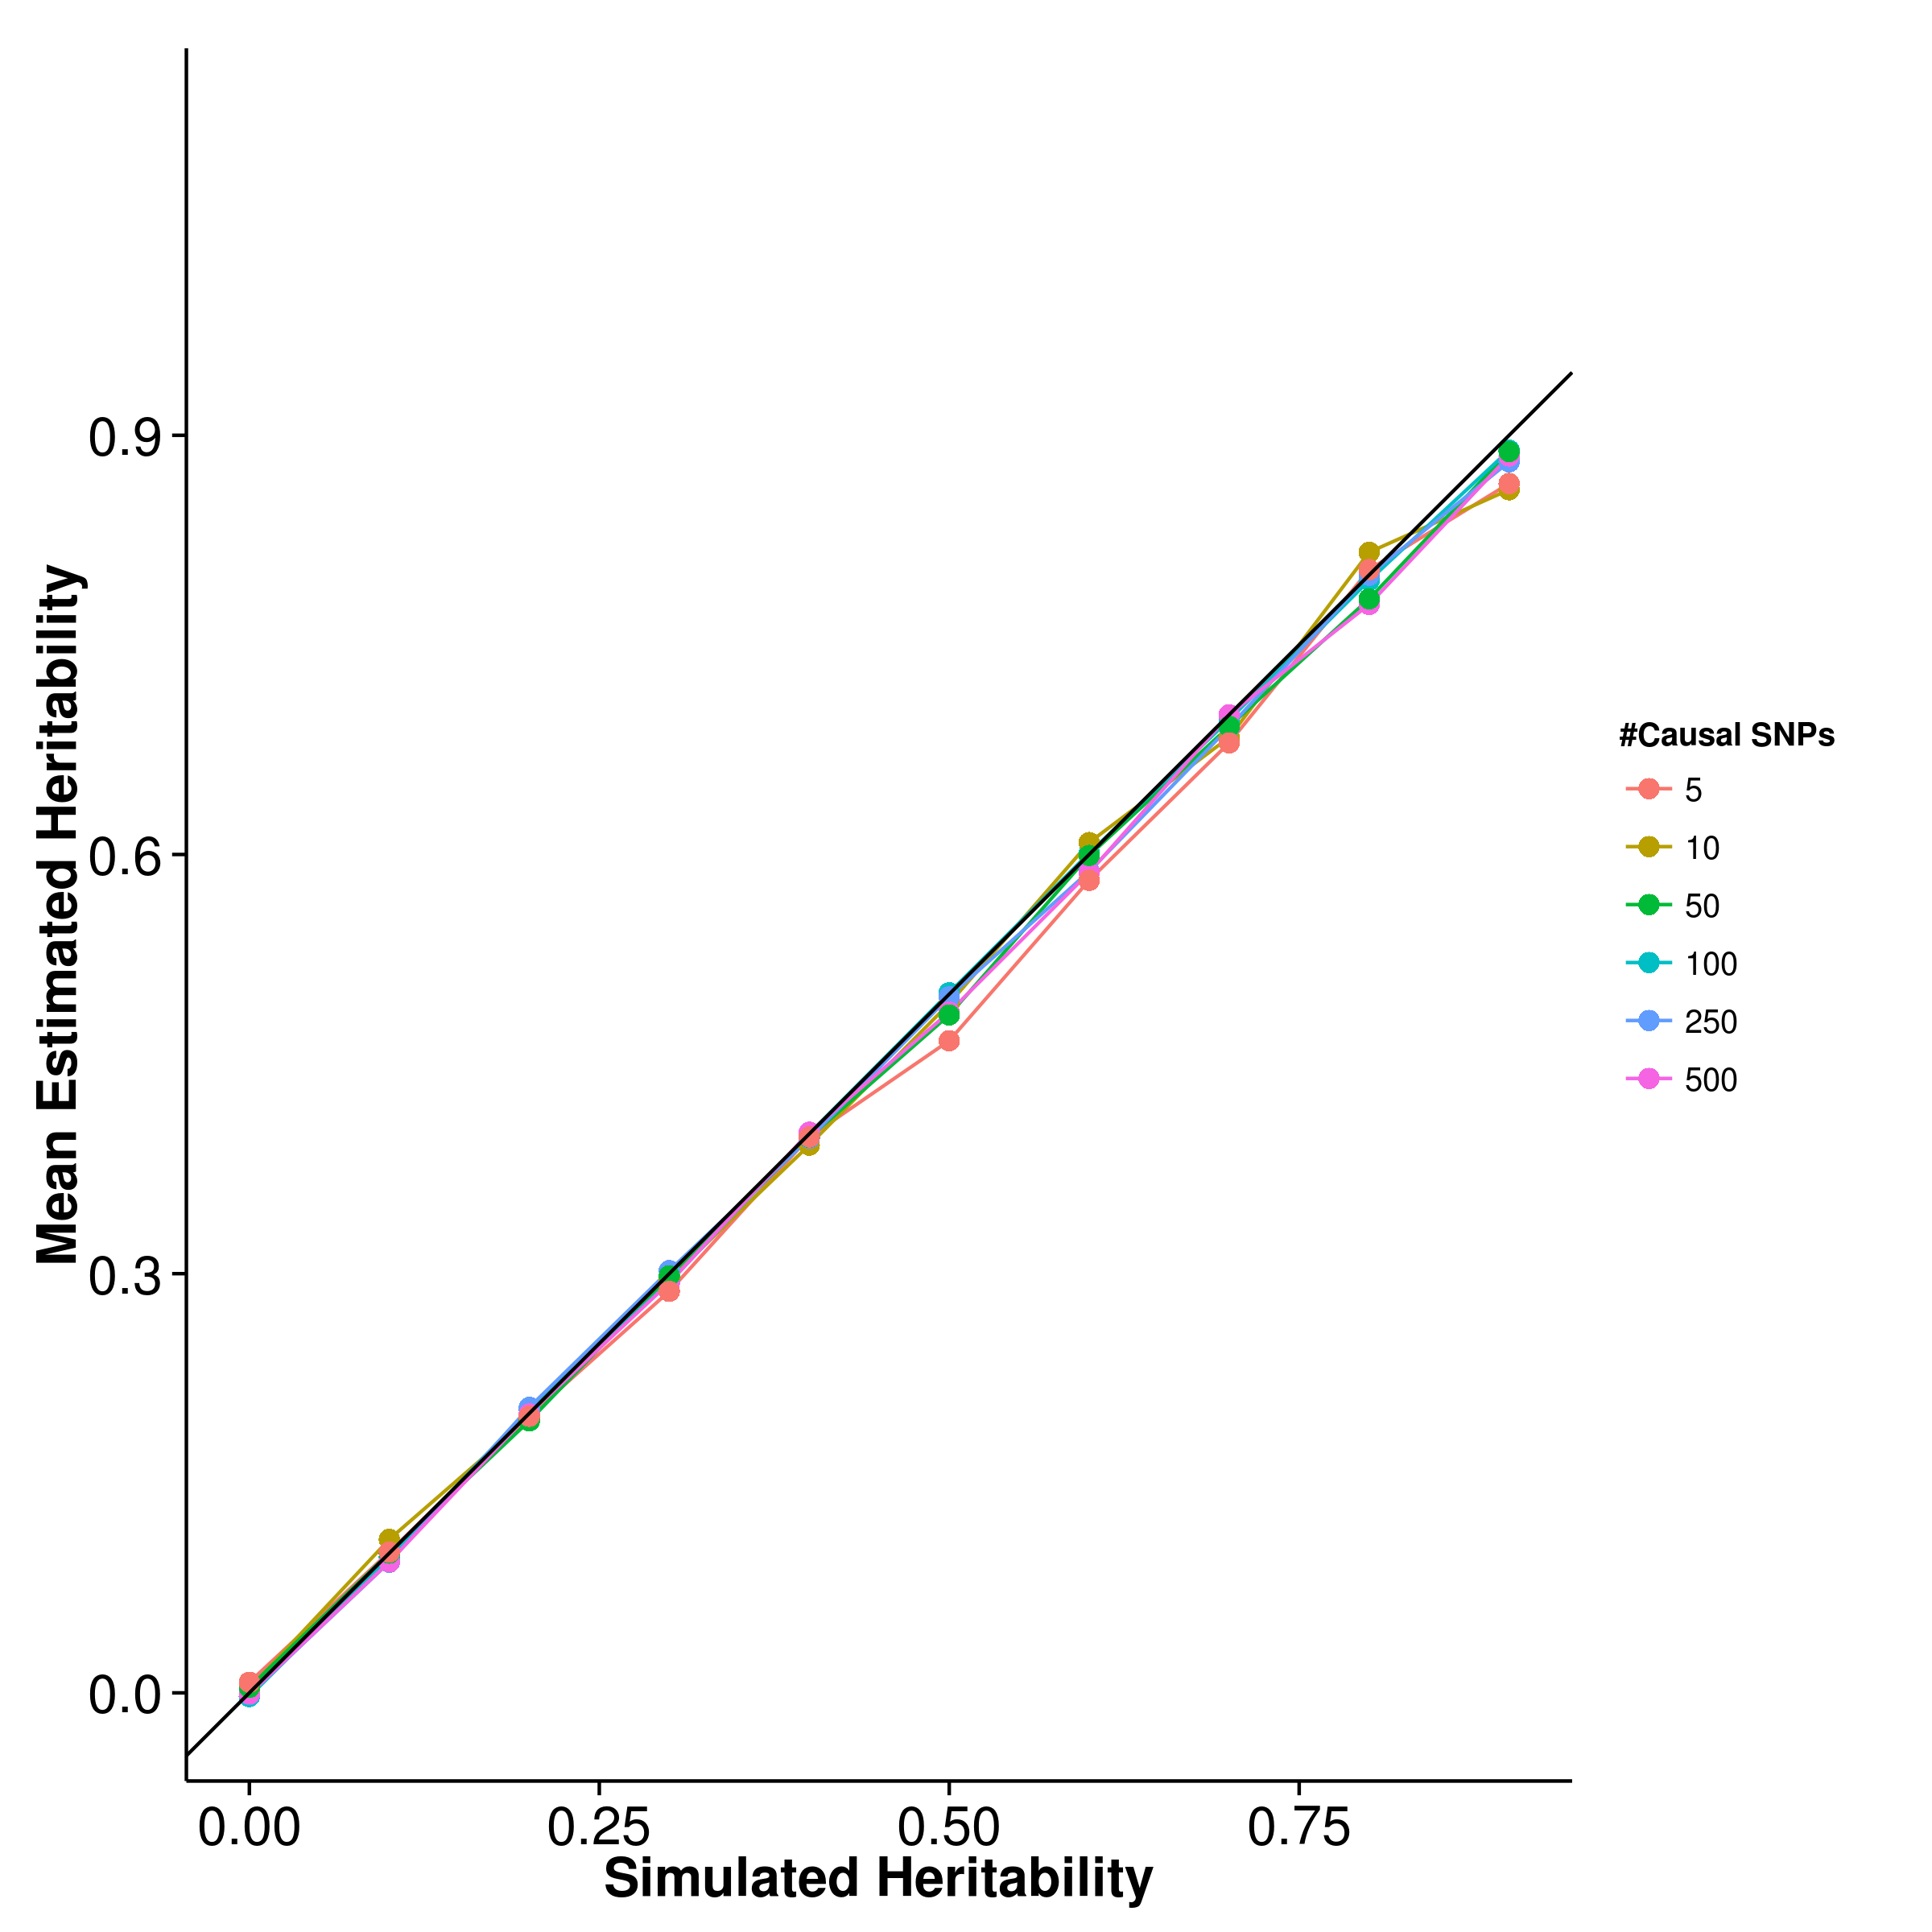
\includegraphics{figure/he_summary/random/shrek_Qt_Random_mean.png}}
				\label{fig:shrekQtRandMean}
			}
			\subfloat[GCTA]{
				\scalebox{.4}{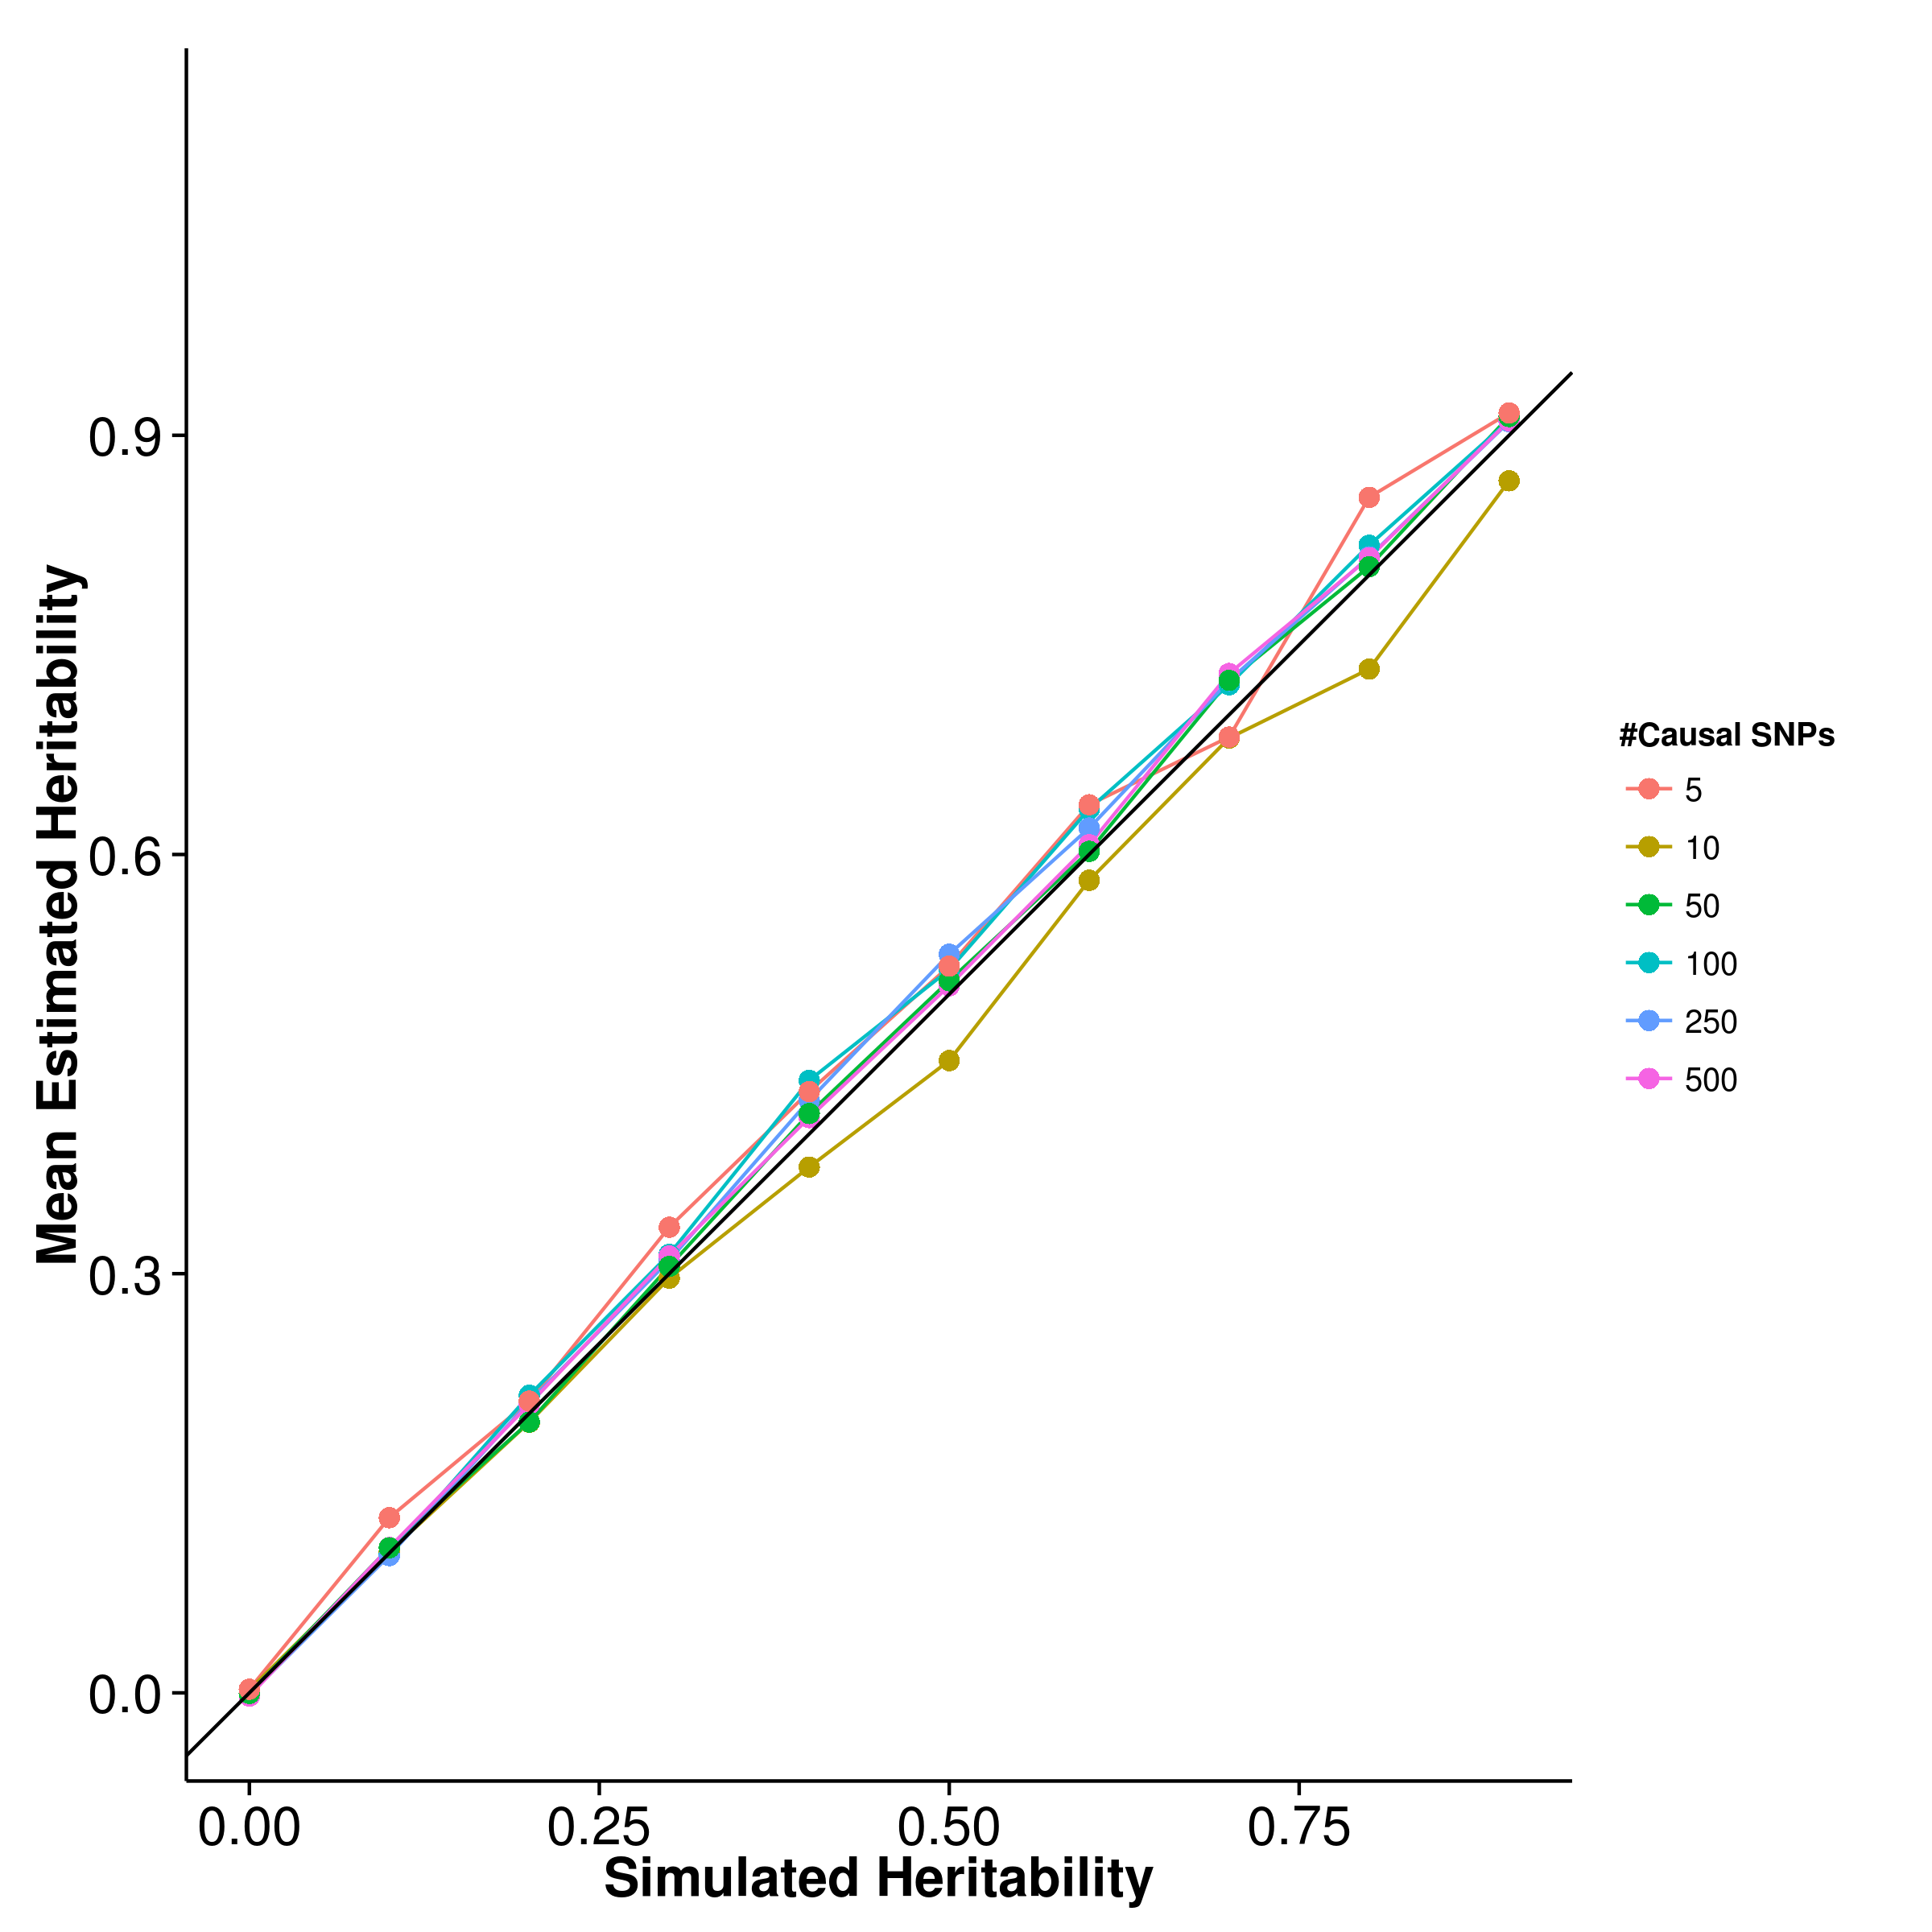
\includegraphics{figure/he_summary/random/gcta_Qt_Random_mean.png}}
				\label{fig:gctaQtRandMean}
			}\\
			\subfloat[LDSC with fix intercept]{
				\scalebox{.4}{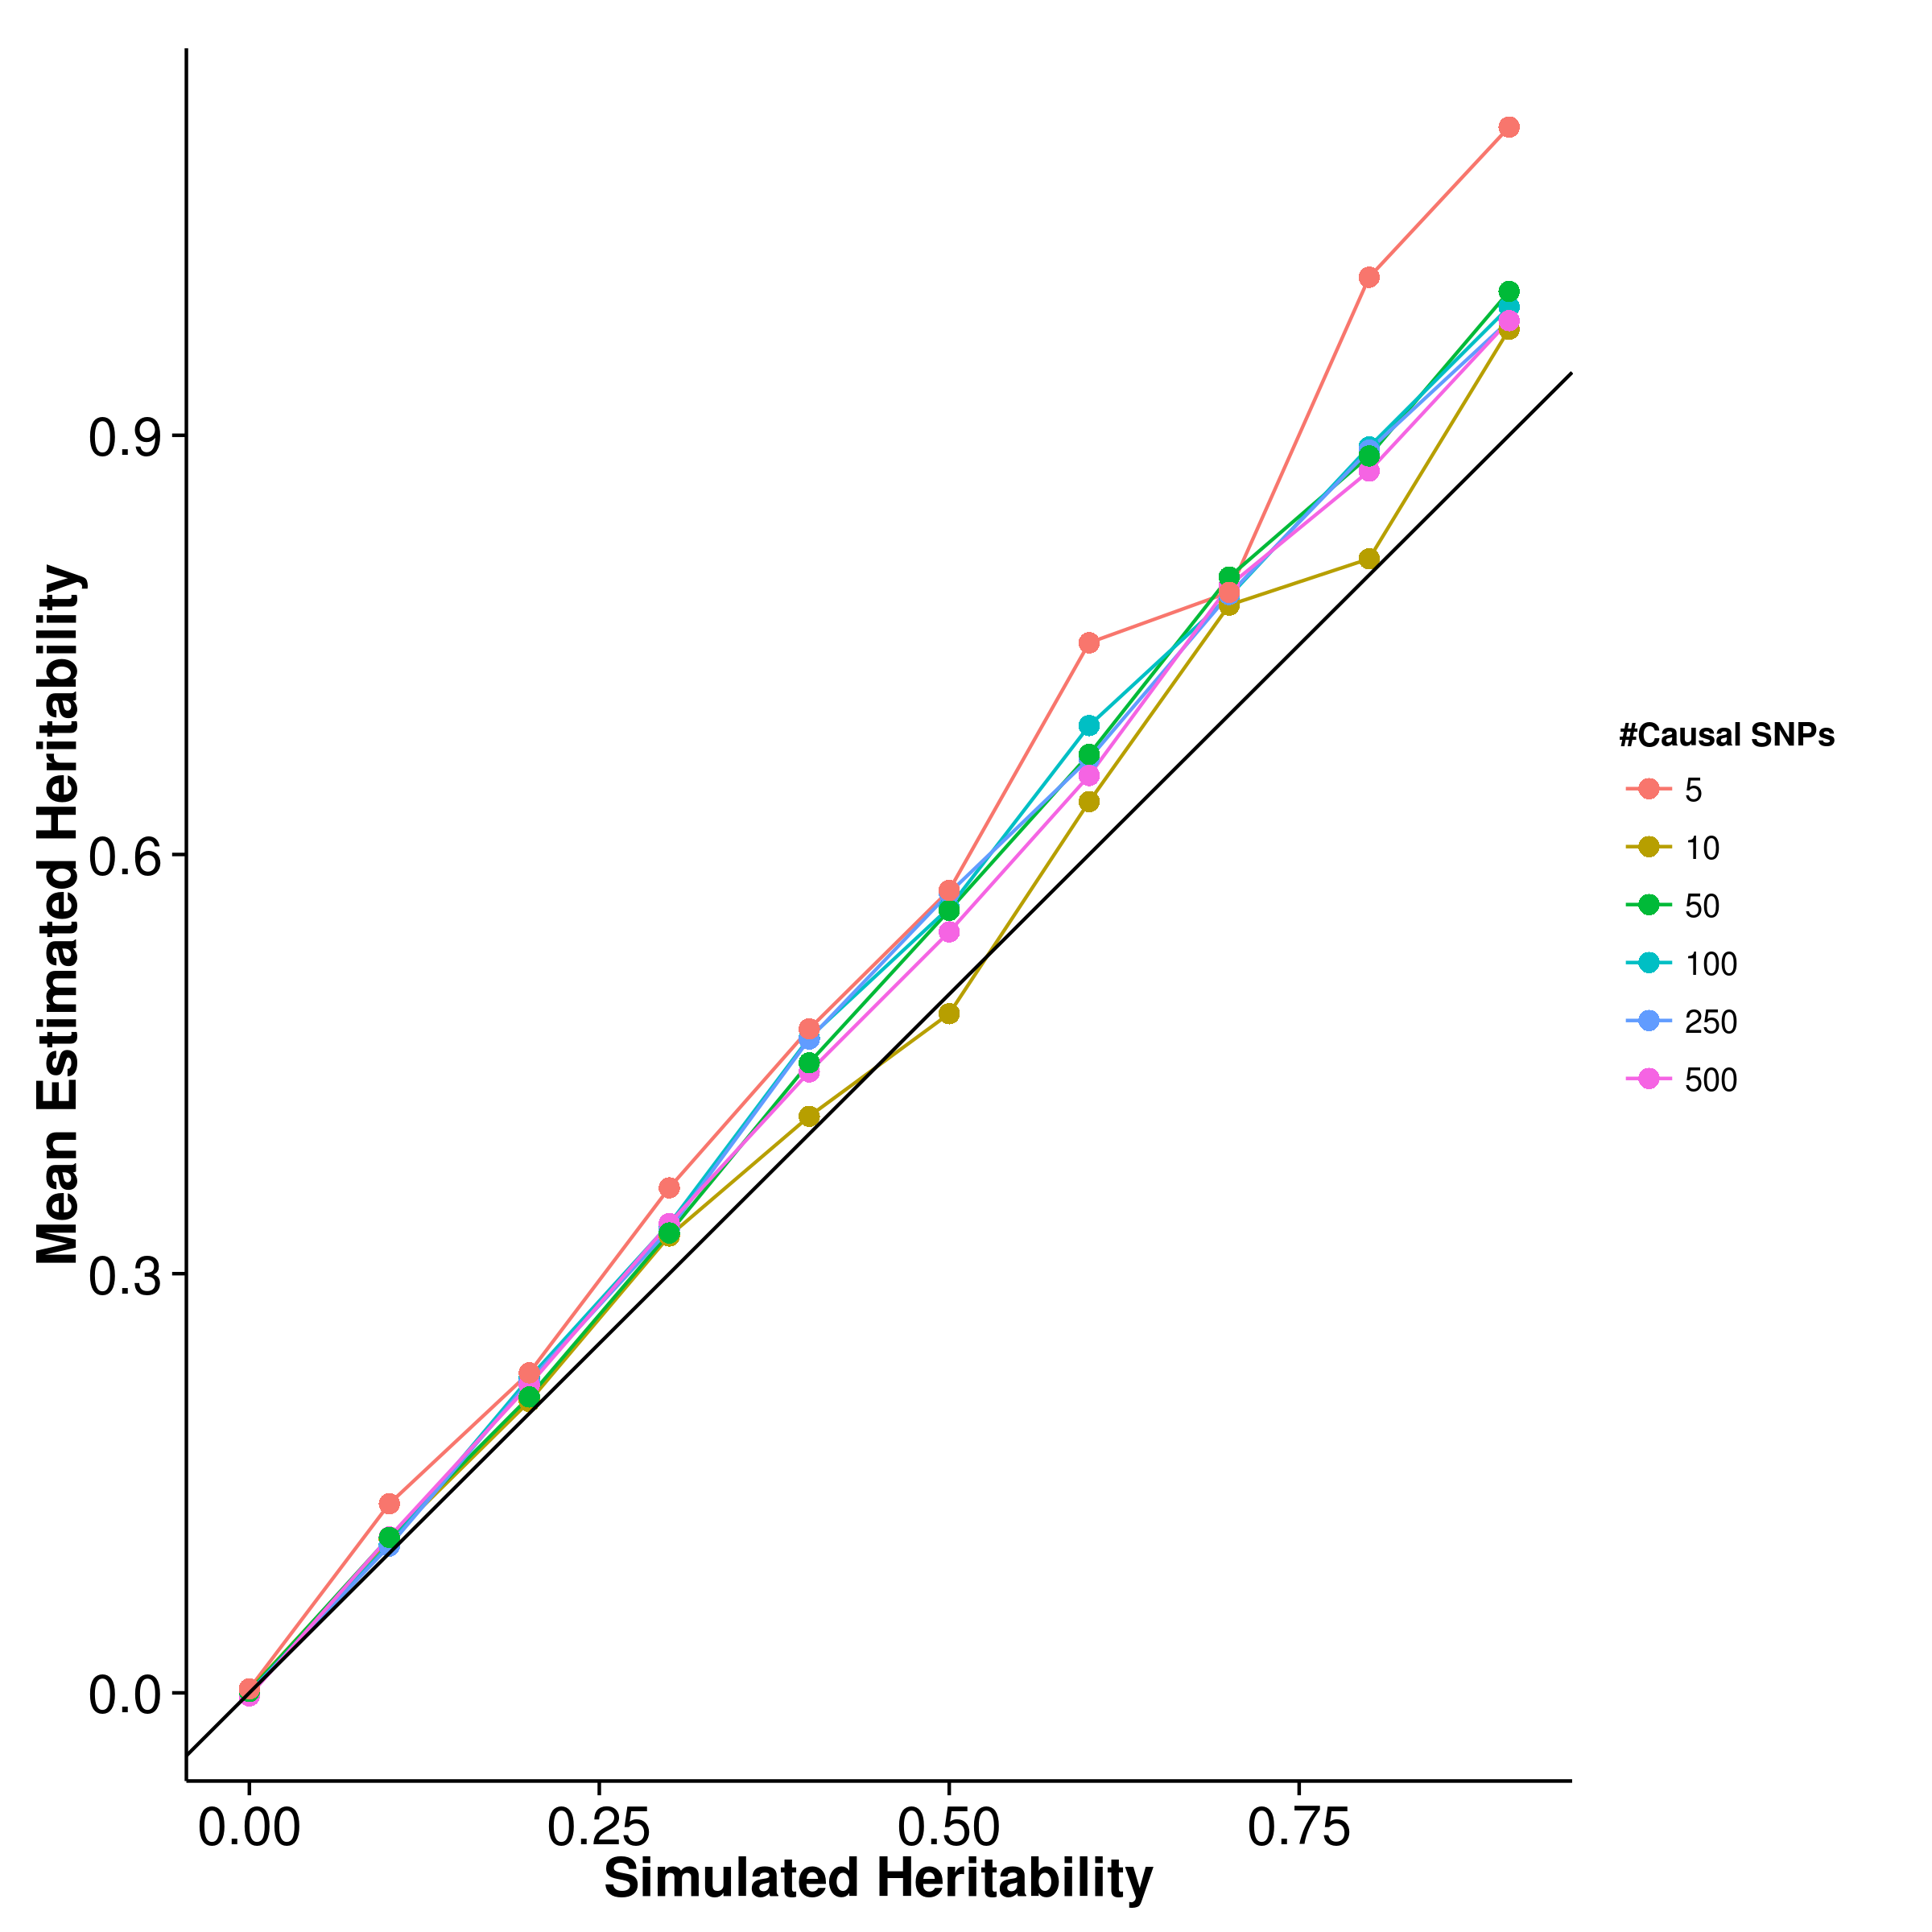
\includegraphics{figure/he_summary/random/ldsc_Qt_Random_mean.png}}
				\label{fig:ldscQtRandMean}
			}
			\subfloat[LDSC with intercept estimation]{
				
				\scalebox{.4}{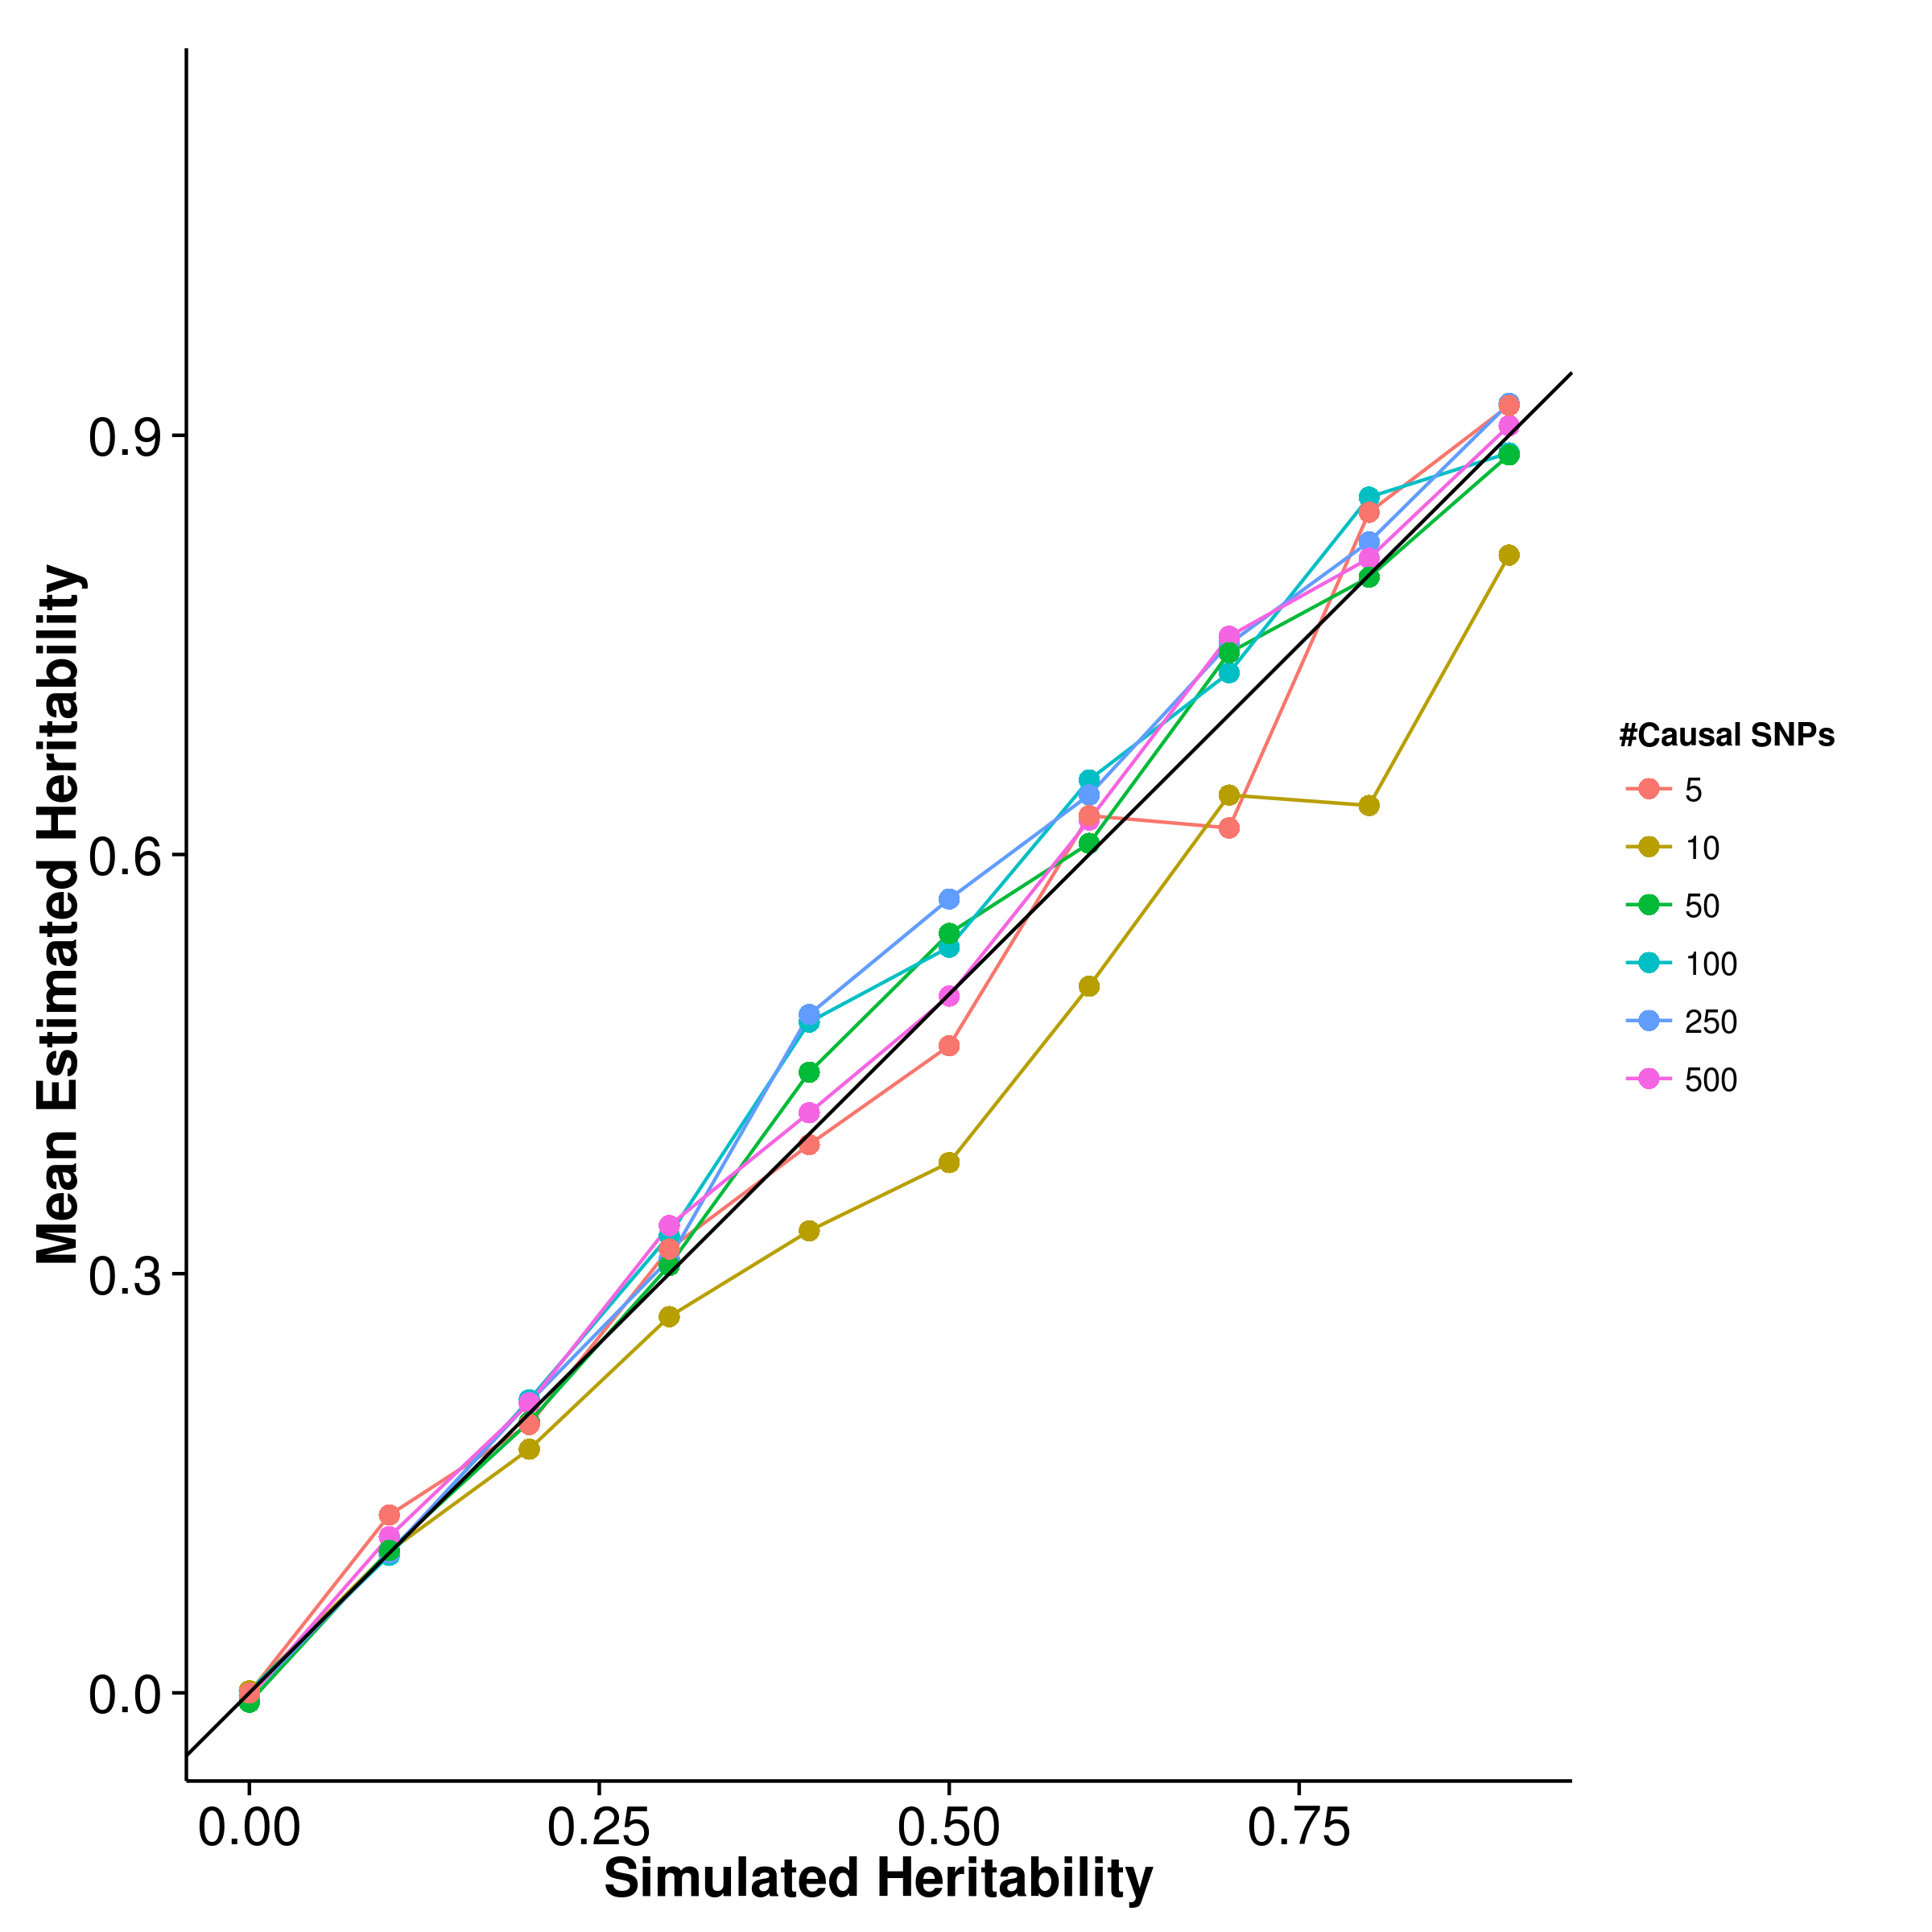
\includegraphics{figure/he_summary/random/ldscIn_Qt_Random_mean.png}}
				\label{fig:ldscInQtRandMean}
			}
			\caption[Quantitative Trait with Random Effect Size Simulation Result(Mean)]
			{Mean of results from quantitative trait simulation with random effect size simulation.
				\gls{shrek} was observed to be slightly biased downward.
				On the other hand, \gls{gcta} were biased upward except in the condition of 10 causal \glspl{SNP}. 
				Whereas a relatively higher upward bias was observed for \gls{ldsc}.} 
			\label{fig:QtRandMean}
		\end{figure}
		
		\begin{figure}
			\centering
			\subfloat[SHREK]{
				\scalebox{.4}{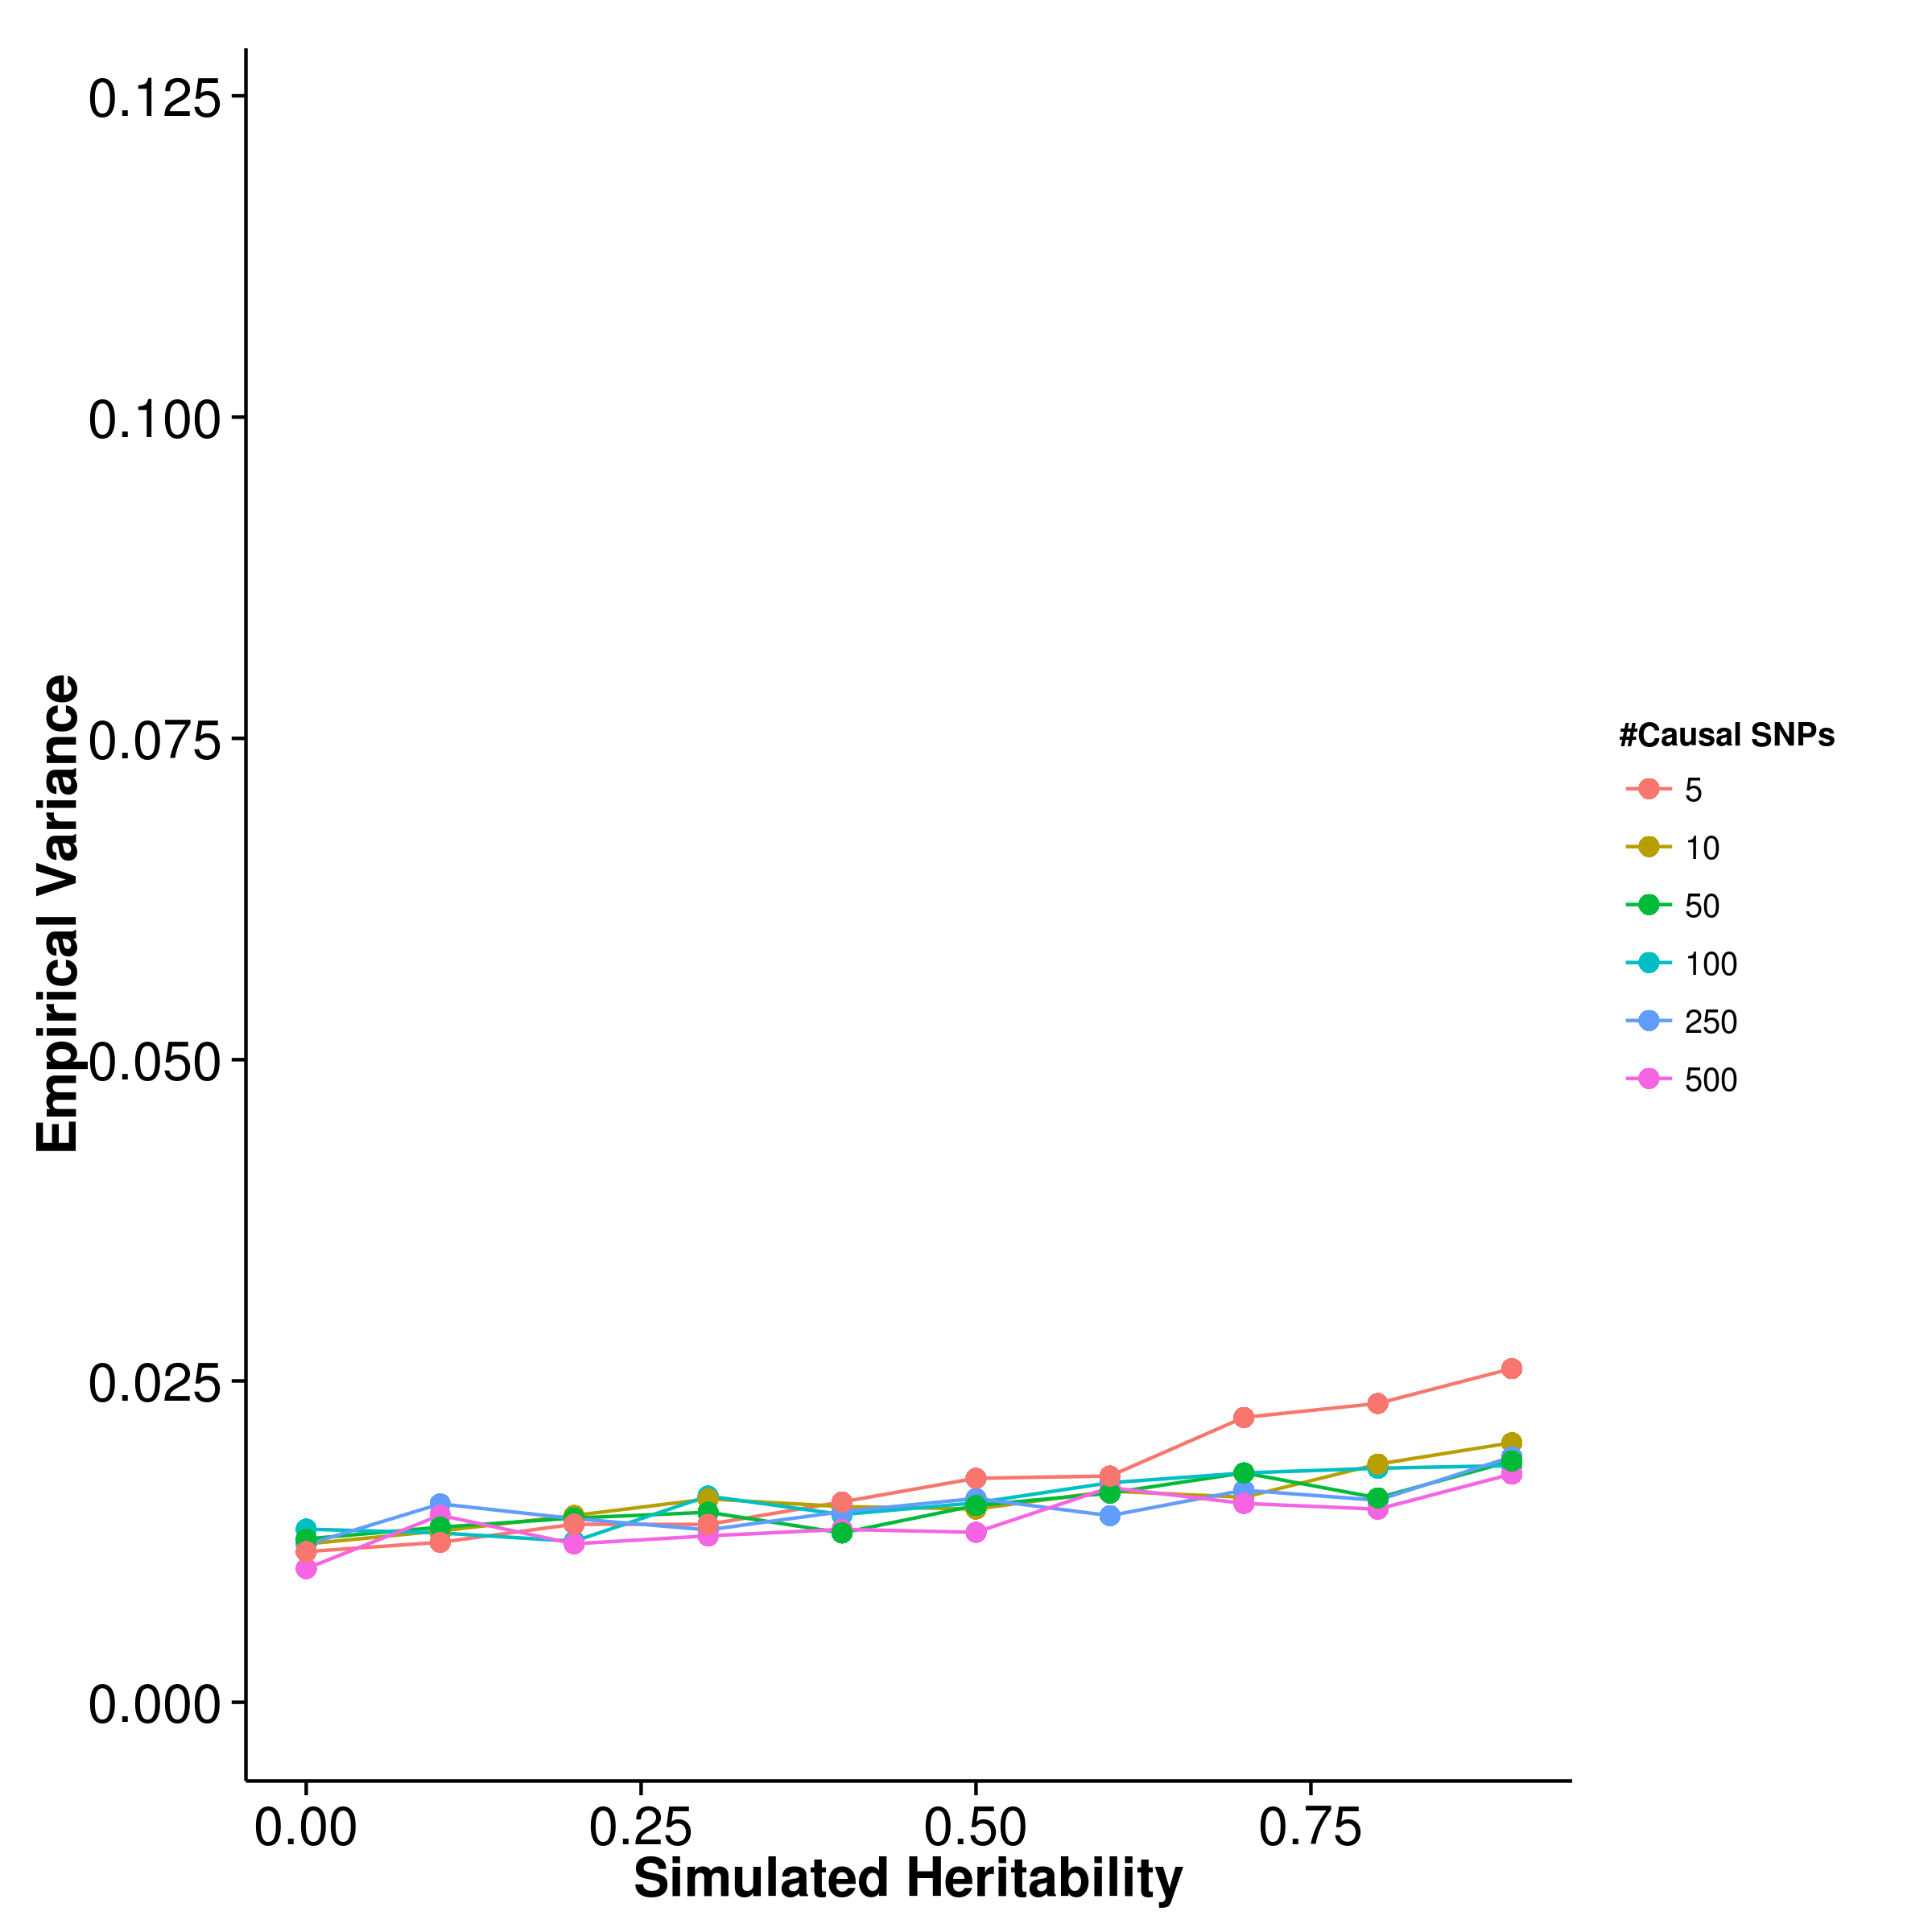
\includegraphics{figure/he_summary/random/shrek_Qt_Random_sd.png}}
				\label{fig:shrekQtRandVar}
			}
			\subfloat[GCTA]{
				\scalebox{.4}{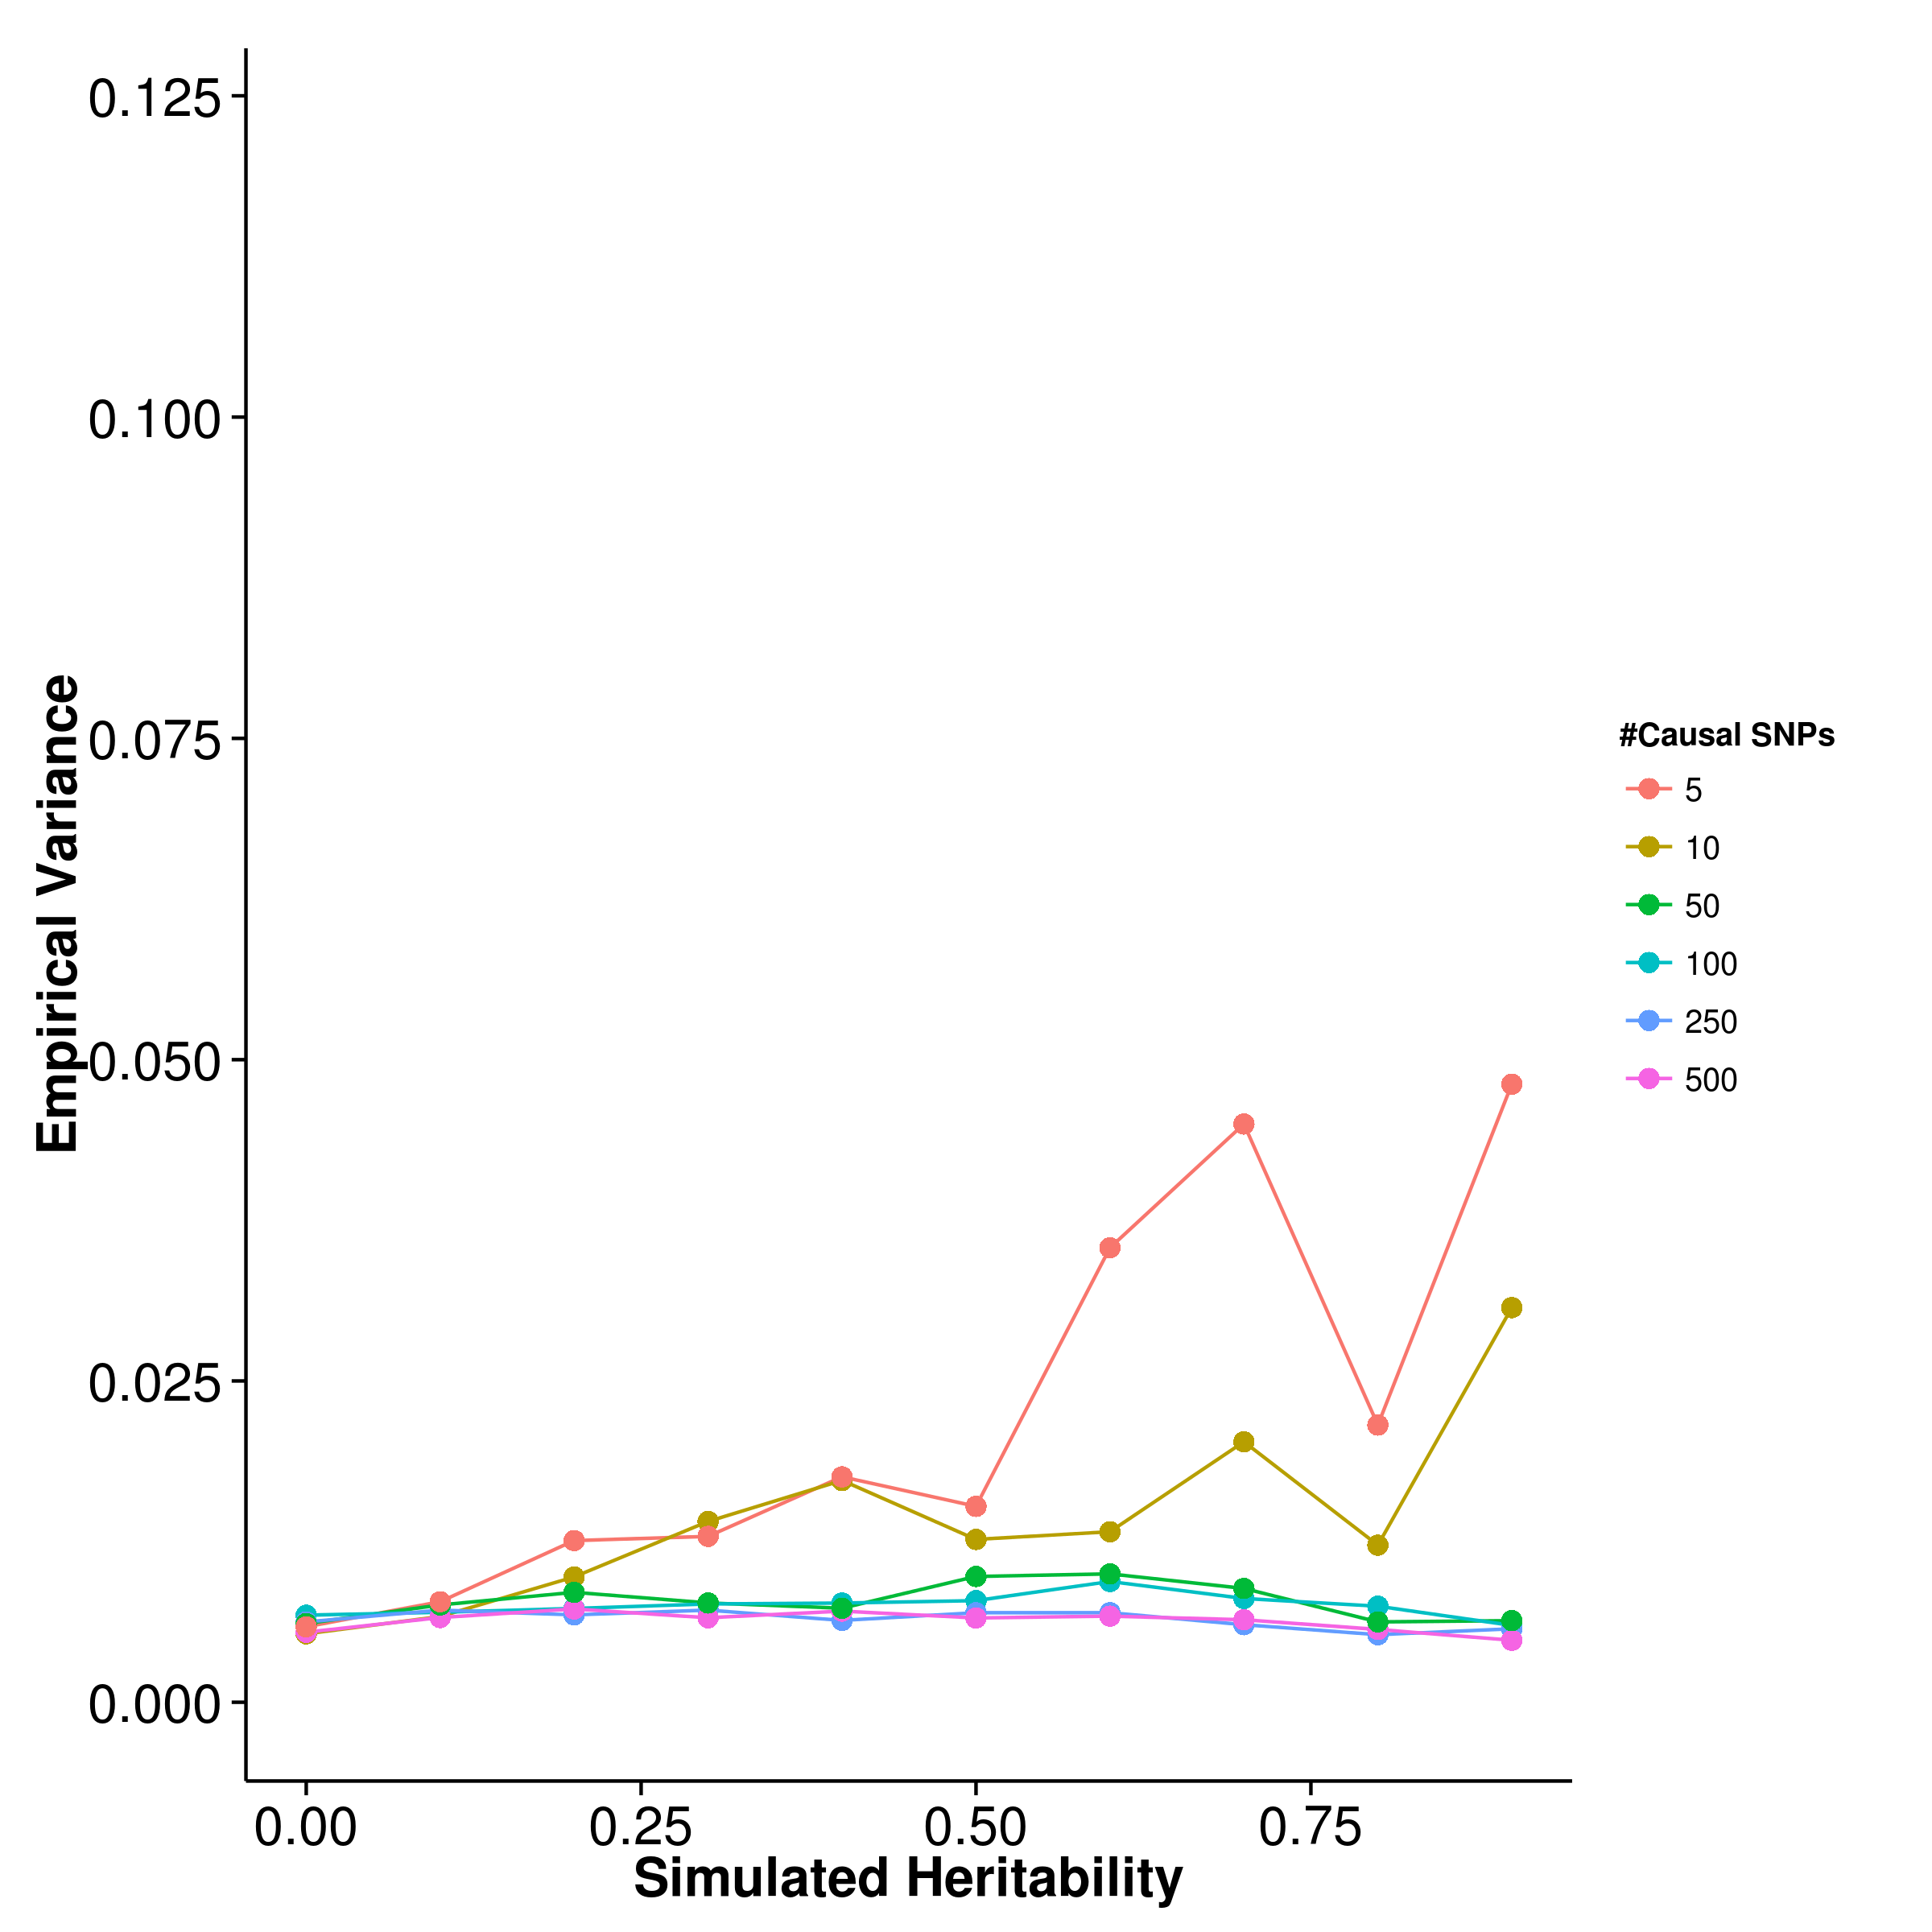
\includegraphics{figure/he_summary/random/gcta_Qt_Random_sd.png}}
				\label{fig:gctaQtRandVar}
			}\\
			\subfloat[LDSC with fix intercept]{
				\scalebox{.4}{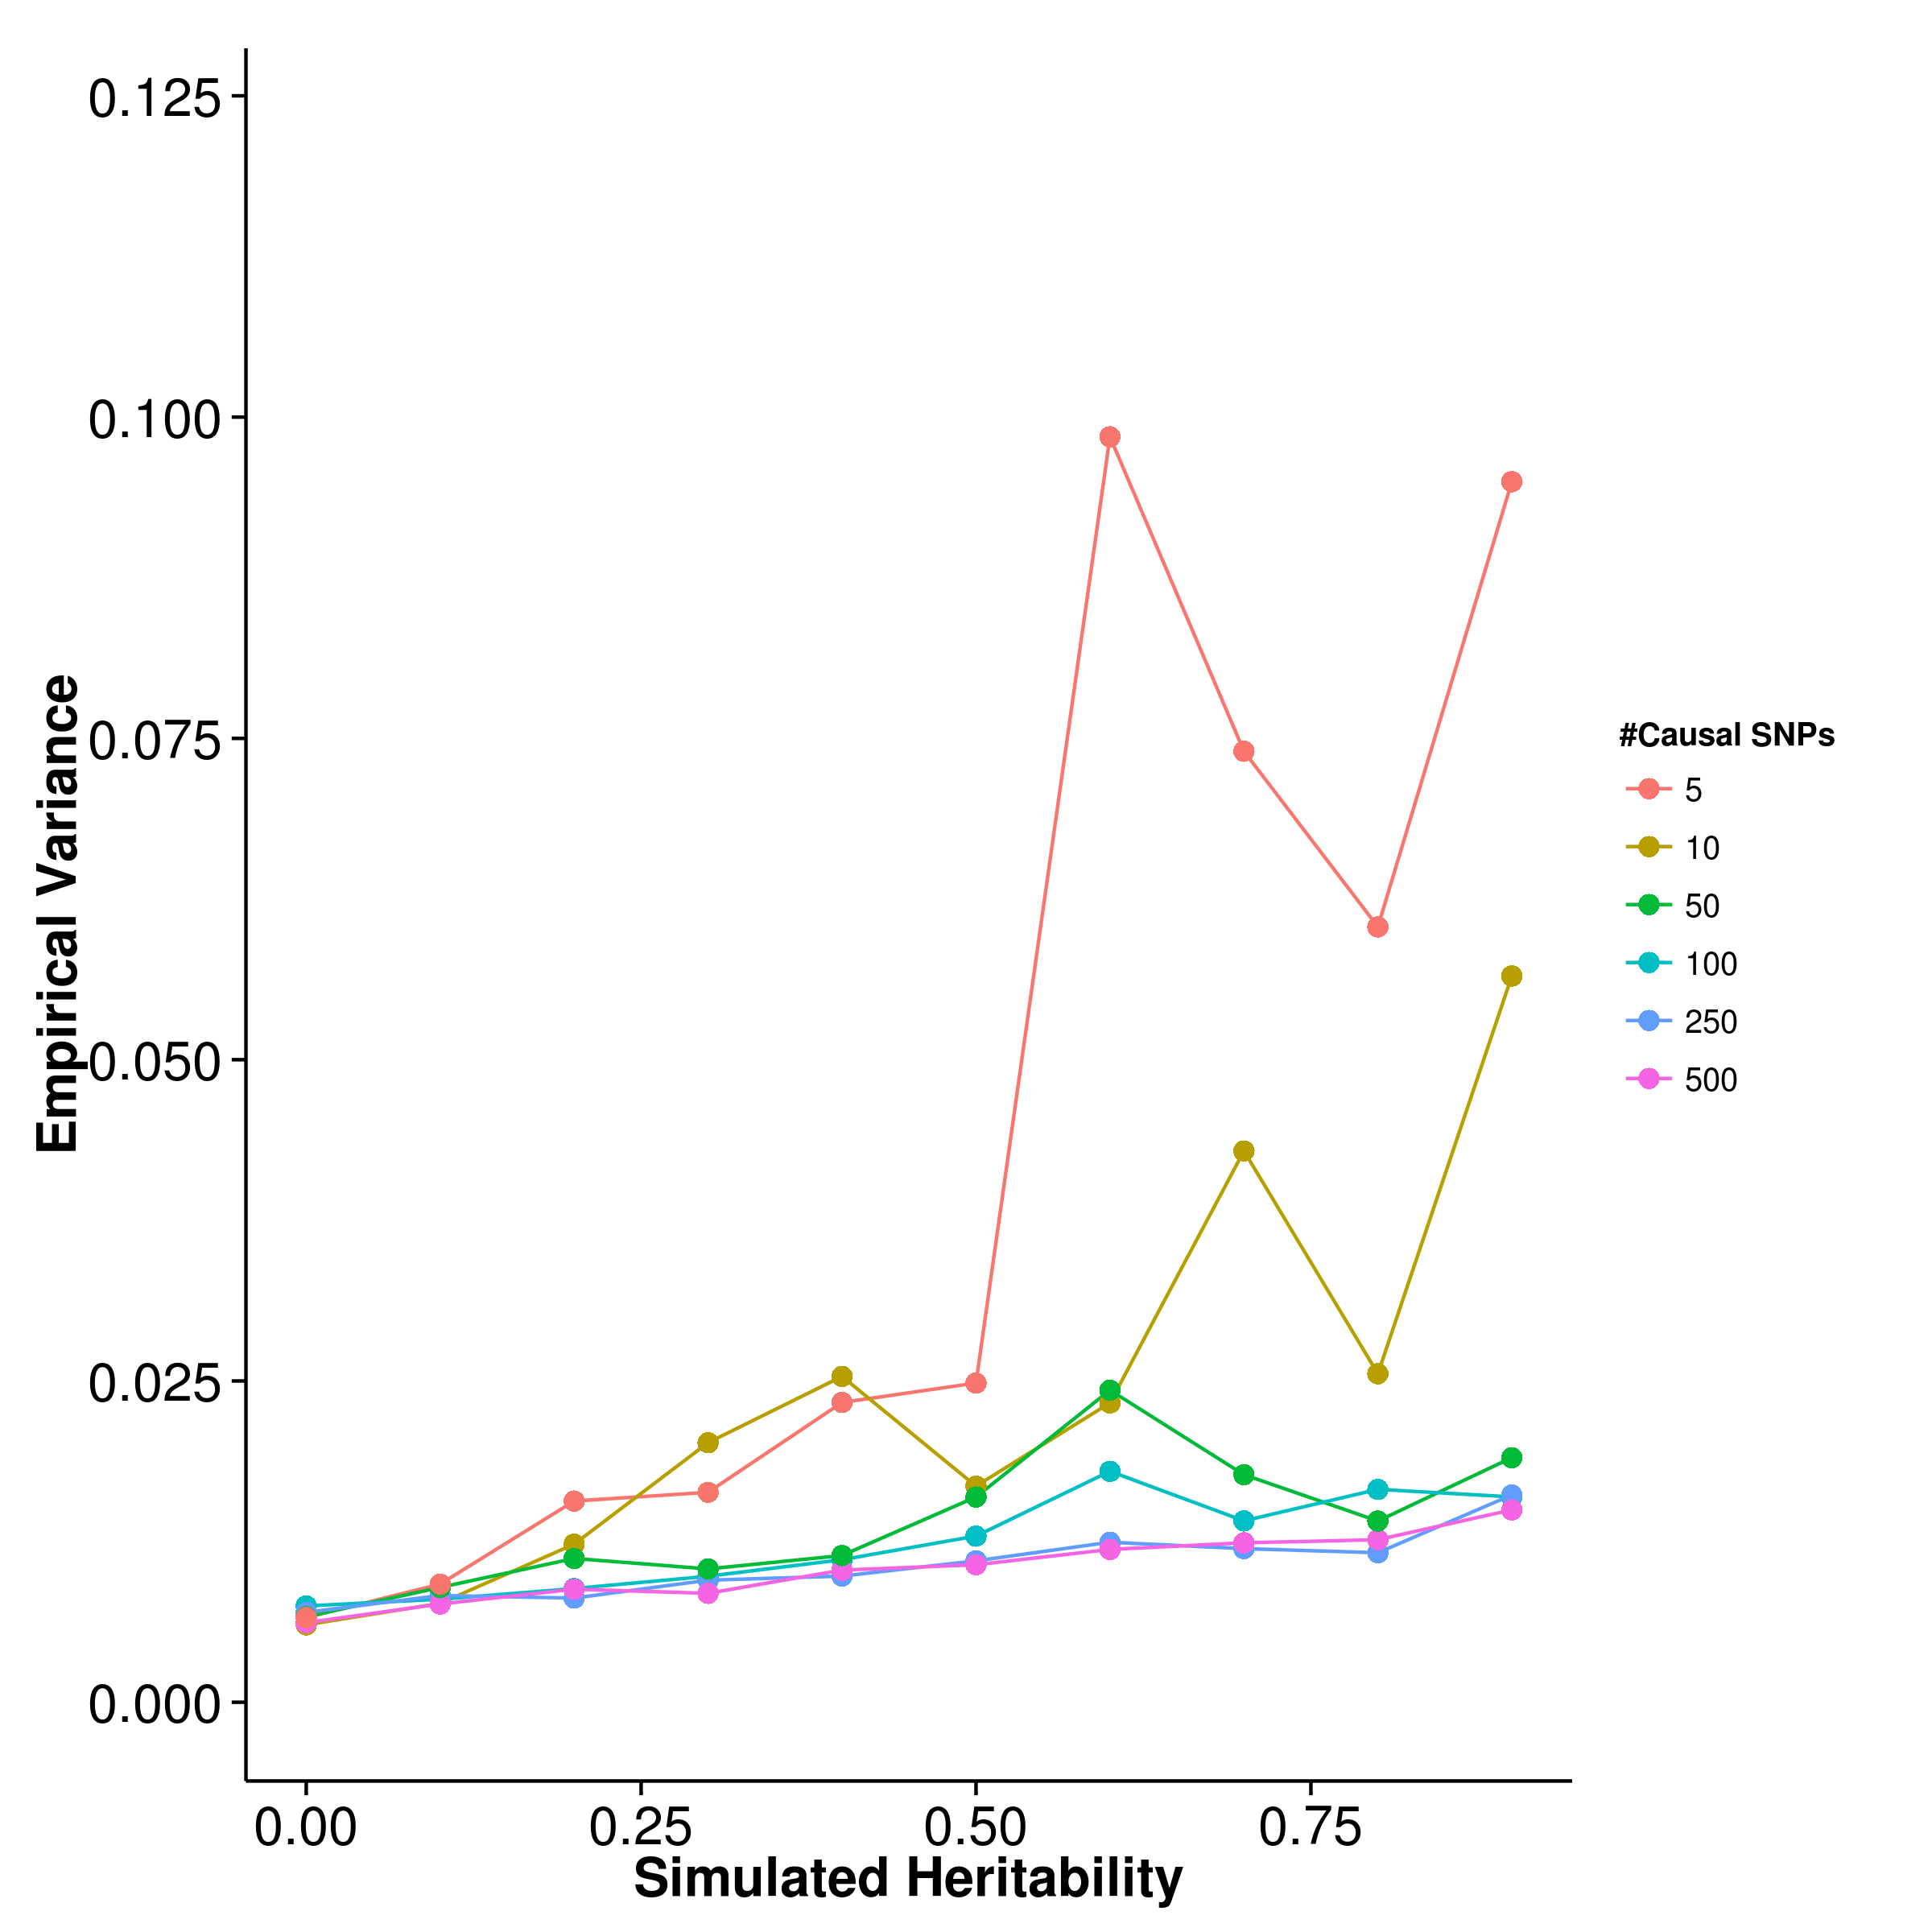
\includegraphics{figure/he_summary/random/ldsc_Qt_Random_sd.png}}
				\label{fig:ldscQtRandVar}
			}
			\subfloat[LDSC with intercept estimation]{
				
				\scalebox{.4}{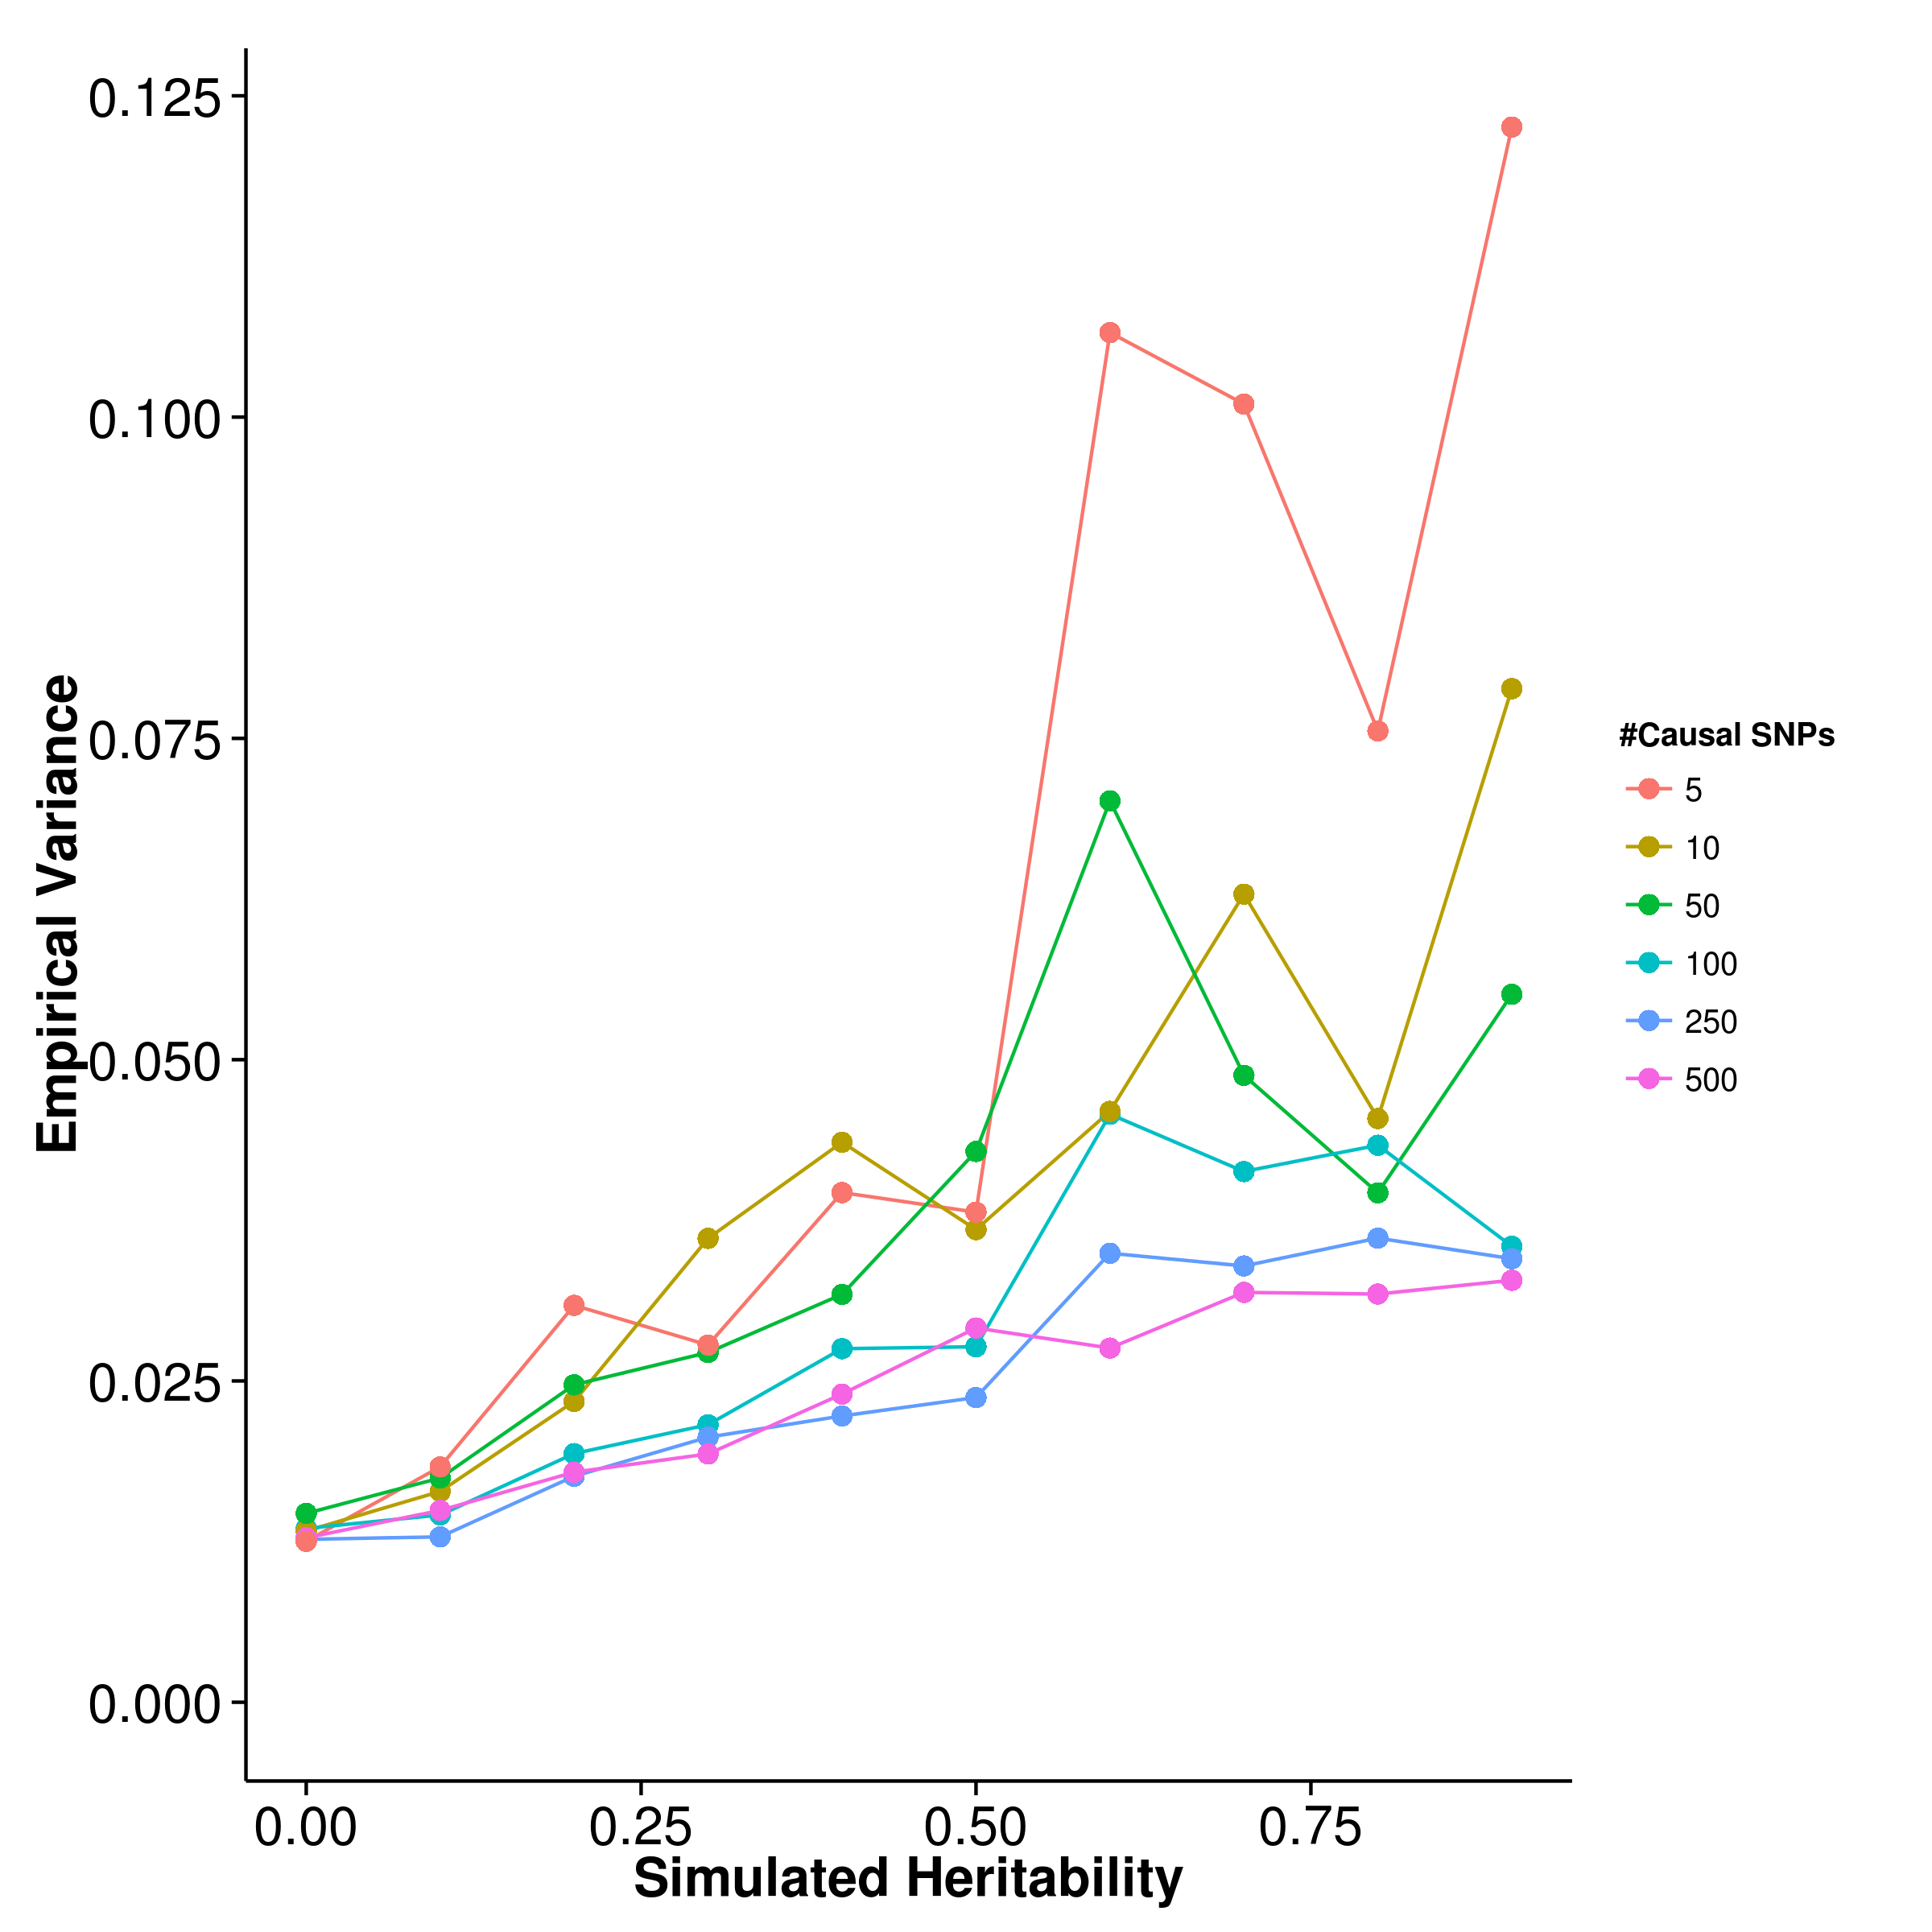
\includegraphics{figure/he_summary/random/ldscIn_Qt_Random_sd.png}}
				\label{fig:ldscInQtRandVar}
			}
			\caption[Quantitative Trait with Random Effect Size Simulation Result(Variance)]
			{Variance of results from quantitative trait simulation with random effect size simulation.
				\gls{gcta} has the smallest variance, follow by \gls{ldsc}. 
				However, it was observed when the number of causal \glspl{SNP} decreases, the variance of the estimation increases for all algorithm, with variance of the \gls{shrek} estimate being the least affected.
			} 
			\label{fig:QtRandVar}
		\end{figure}
		
		\begin{figure}
			\centering
			\subfloat[SHREK]{
				\scalebox{.4}{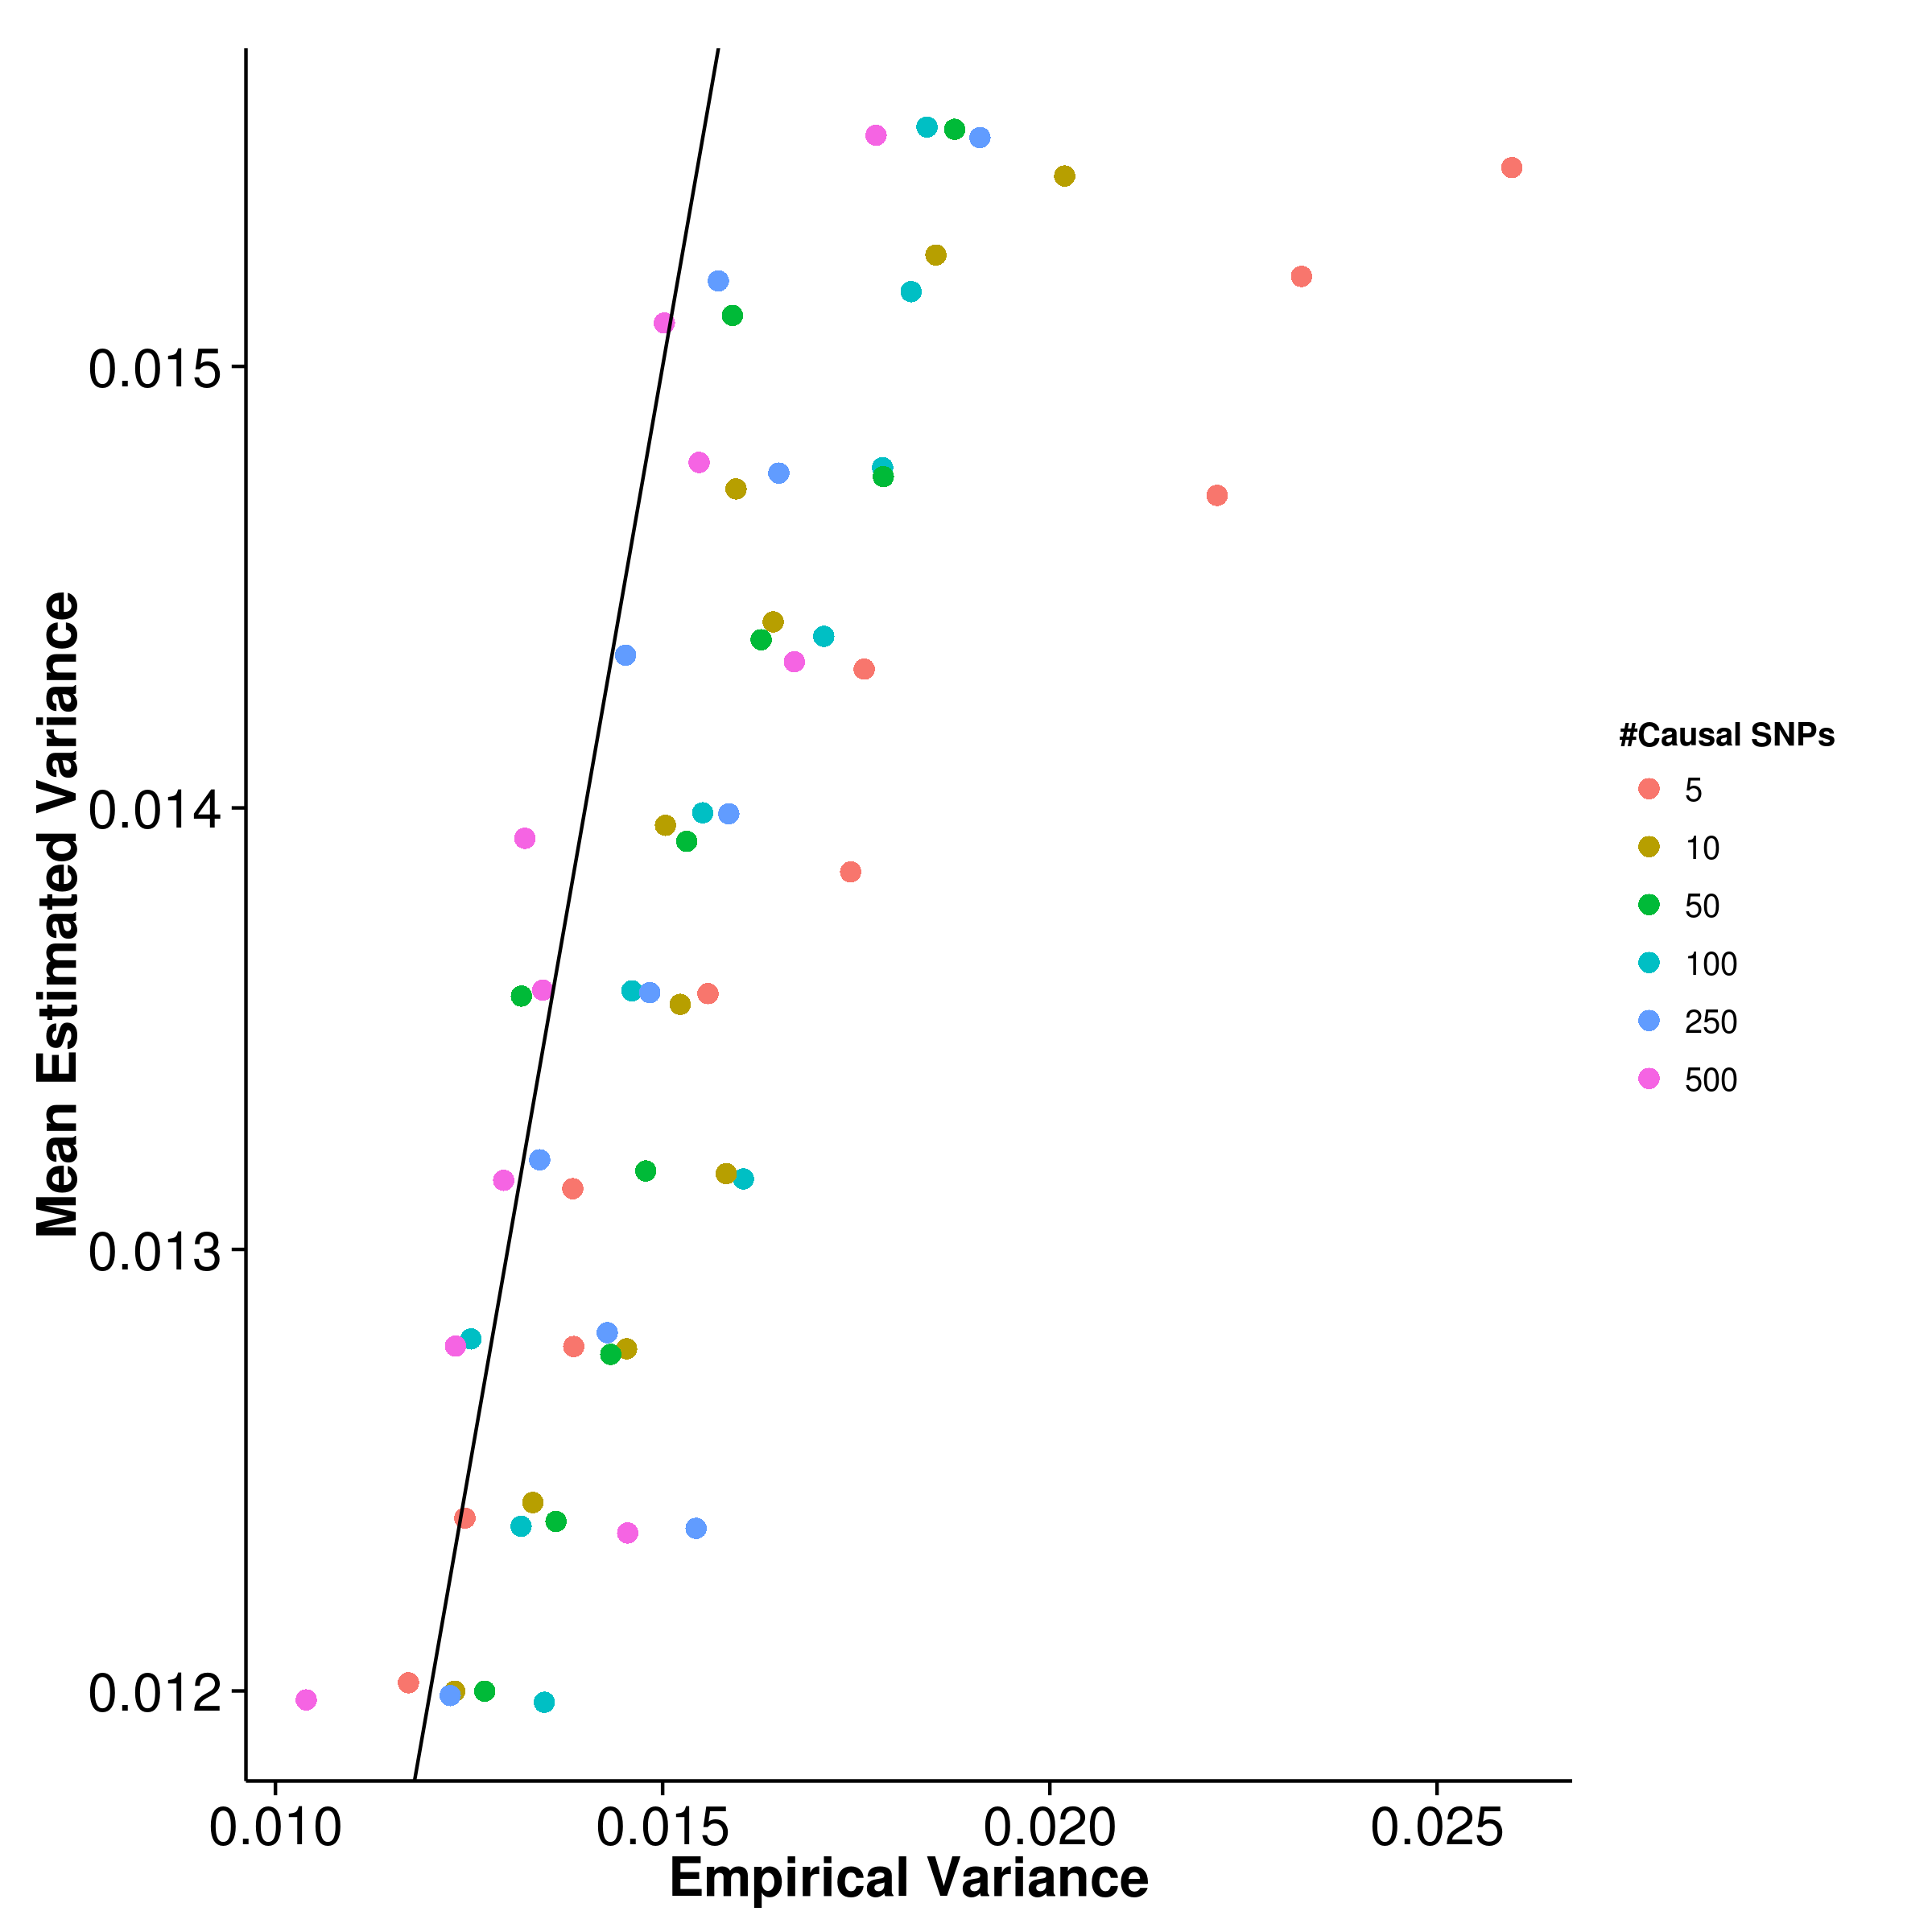
\includegraphics{figure/he_summary/random/shrek_Qt_Random_sdCom.png}}
				\label{fig:shrekQtRandVarCom}
			}
			\subfloat[GCTA]{
				\scalebox{.4}{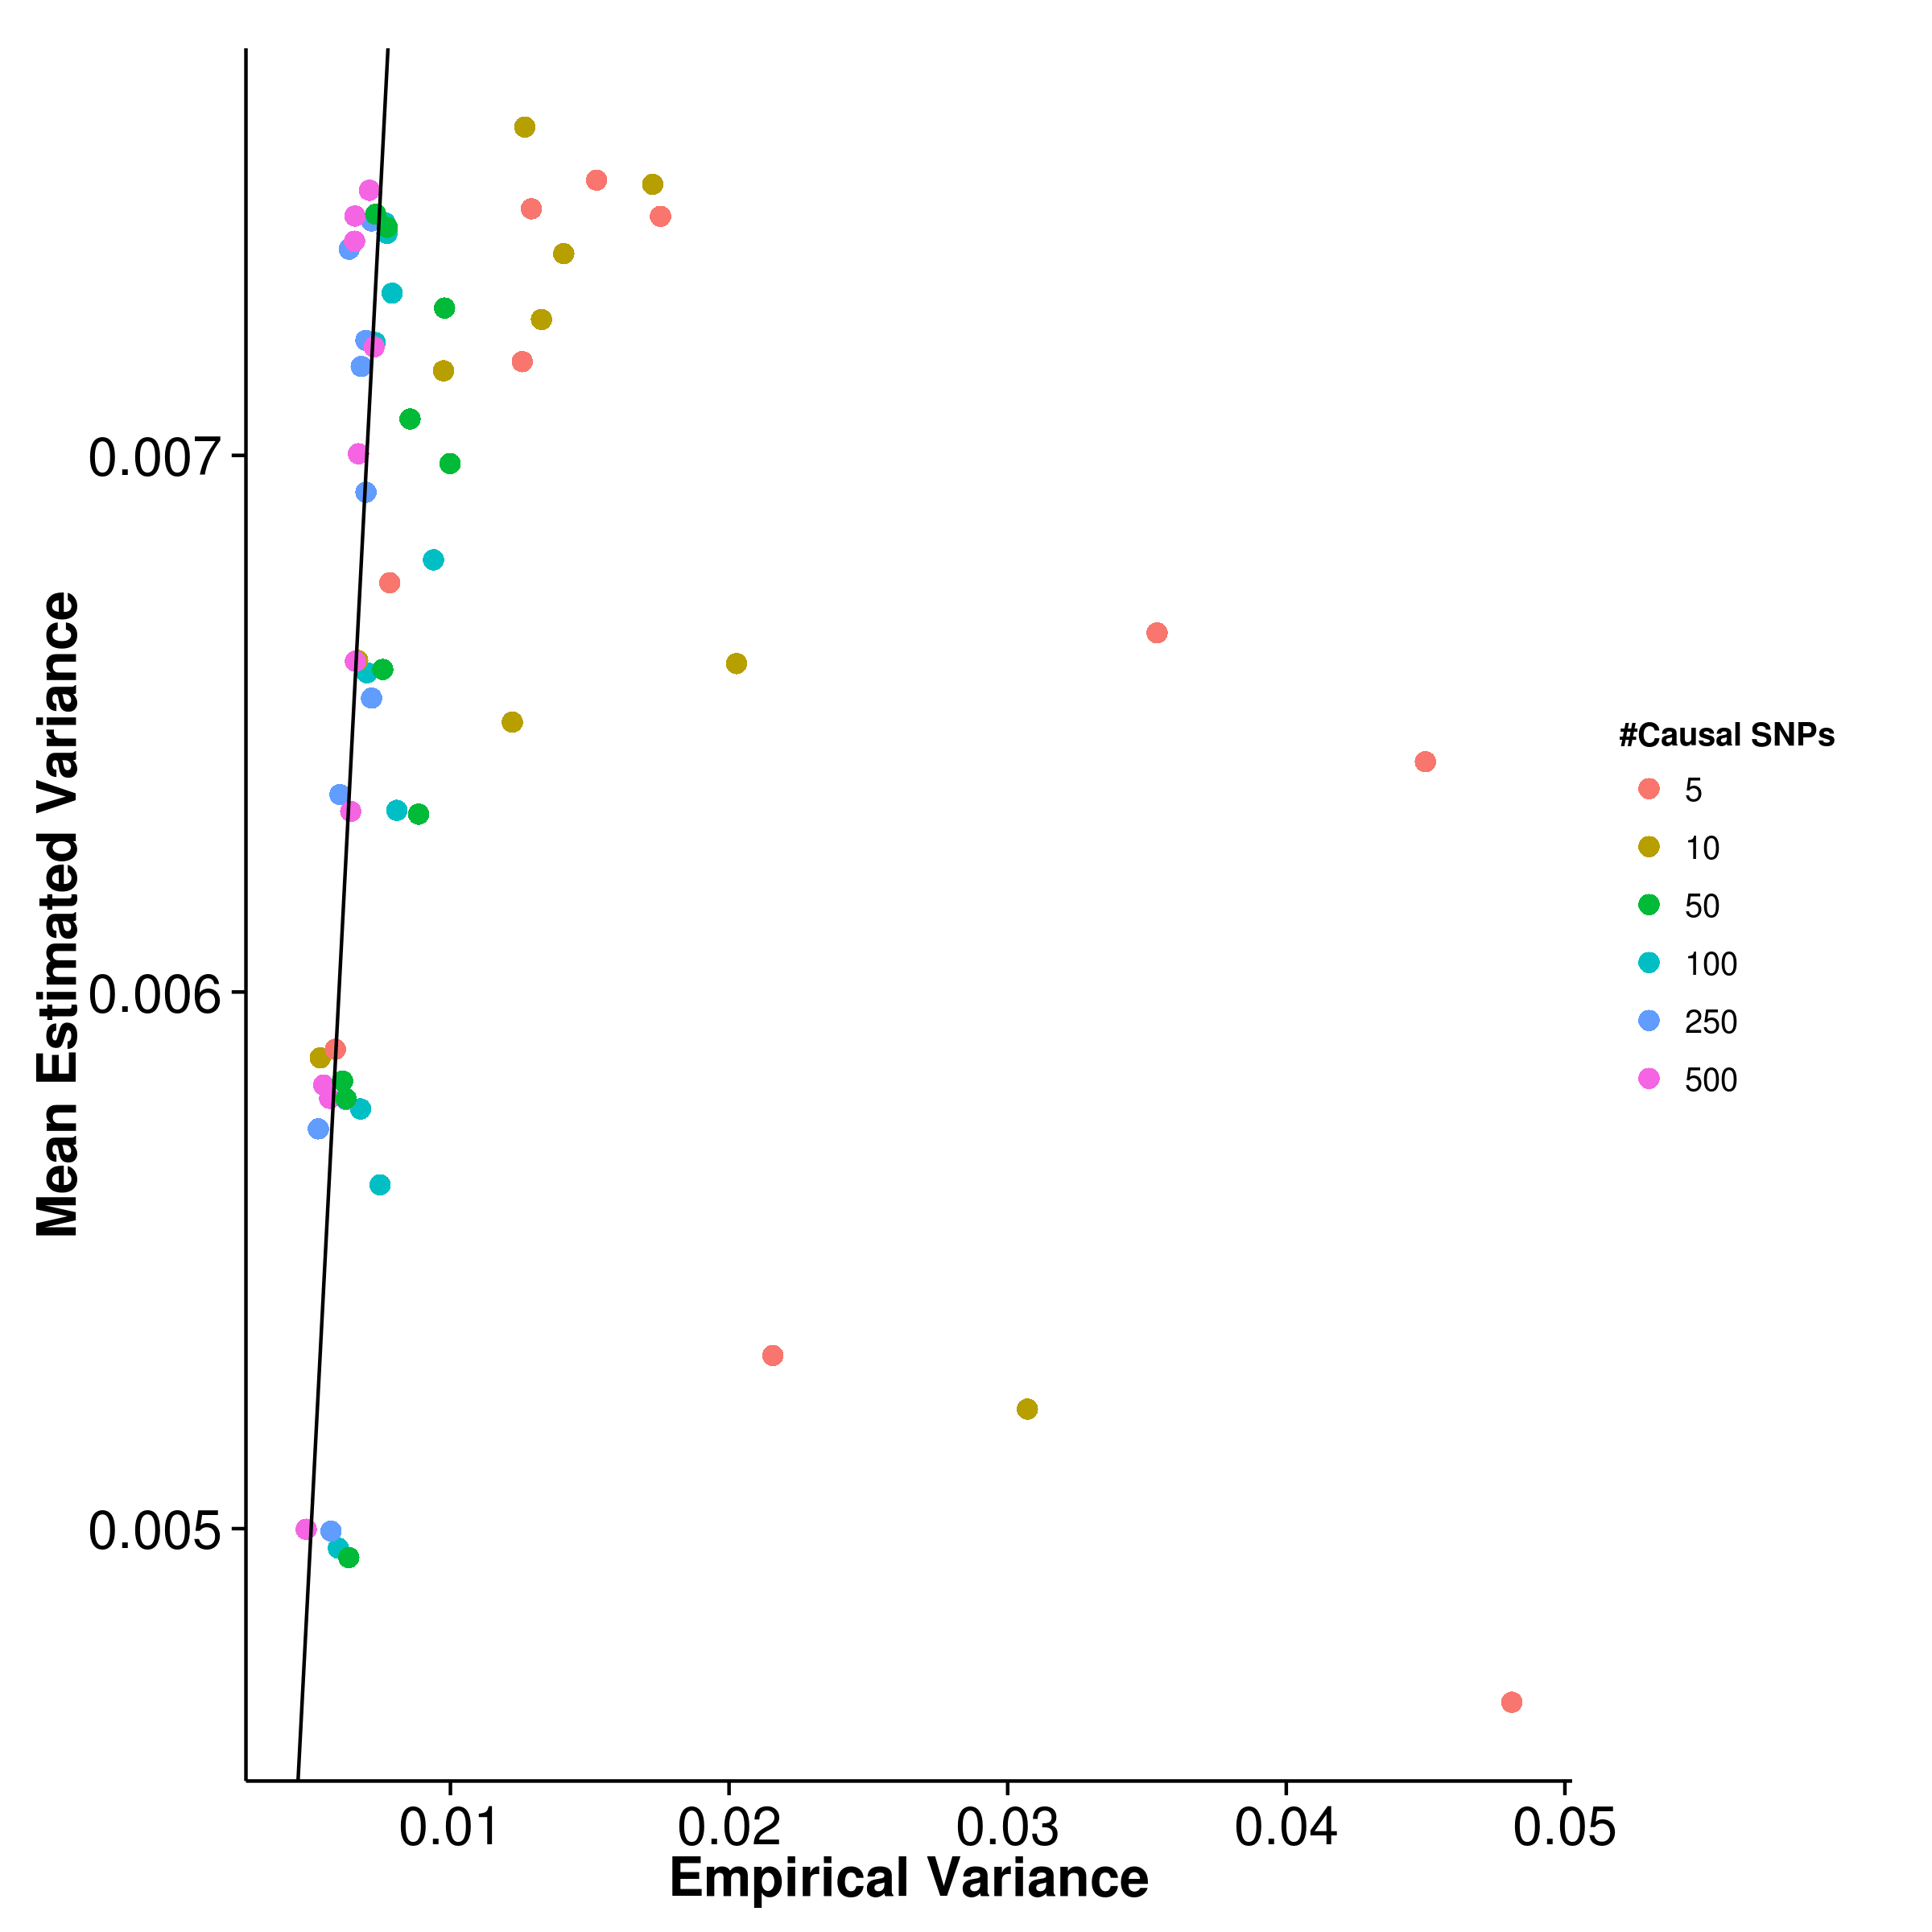
\includegraphics{figure/he_summary/random/gcta_Qt_Random_sdCom.png}}
				\label{fig:gctaQtRandVarCom}
			}\\
			\subfloat[LDSC with fix intercept]{
				\scalebox{.4}{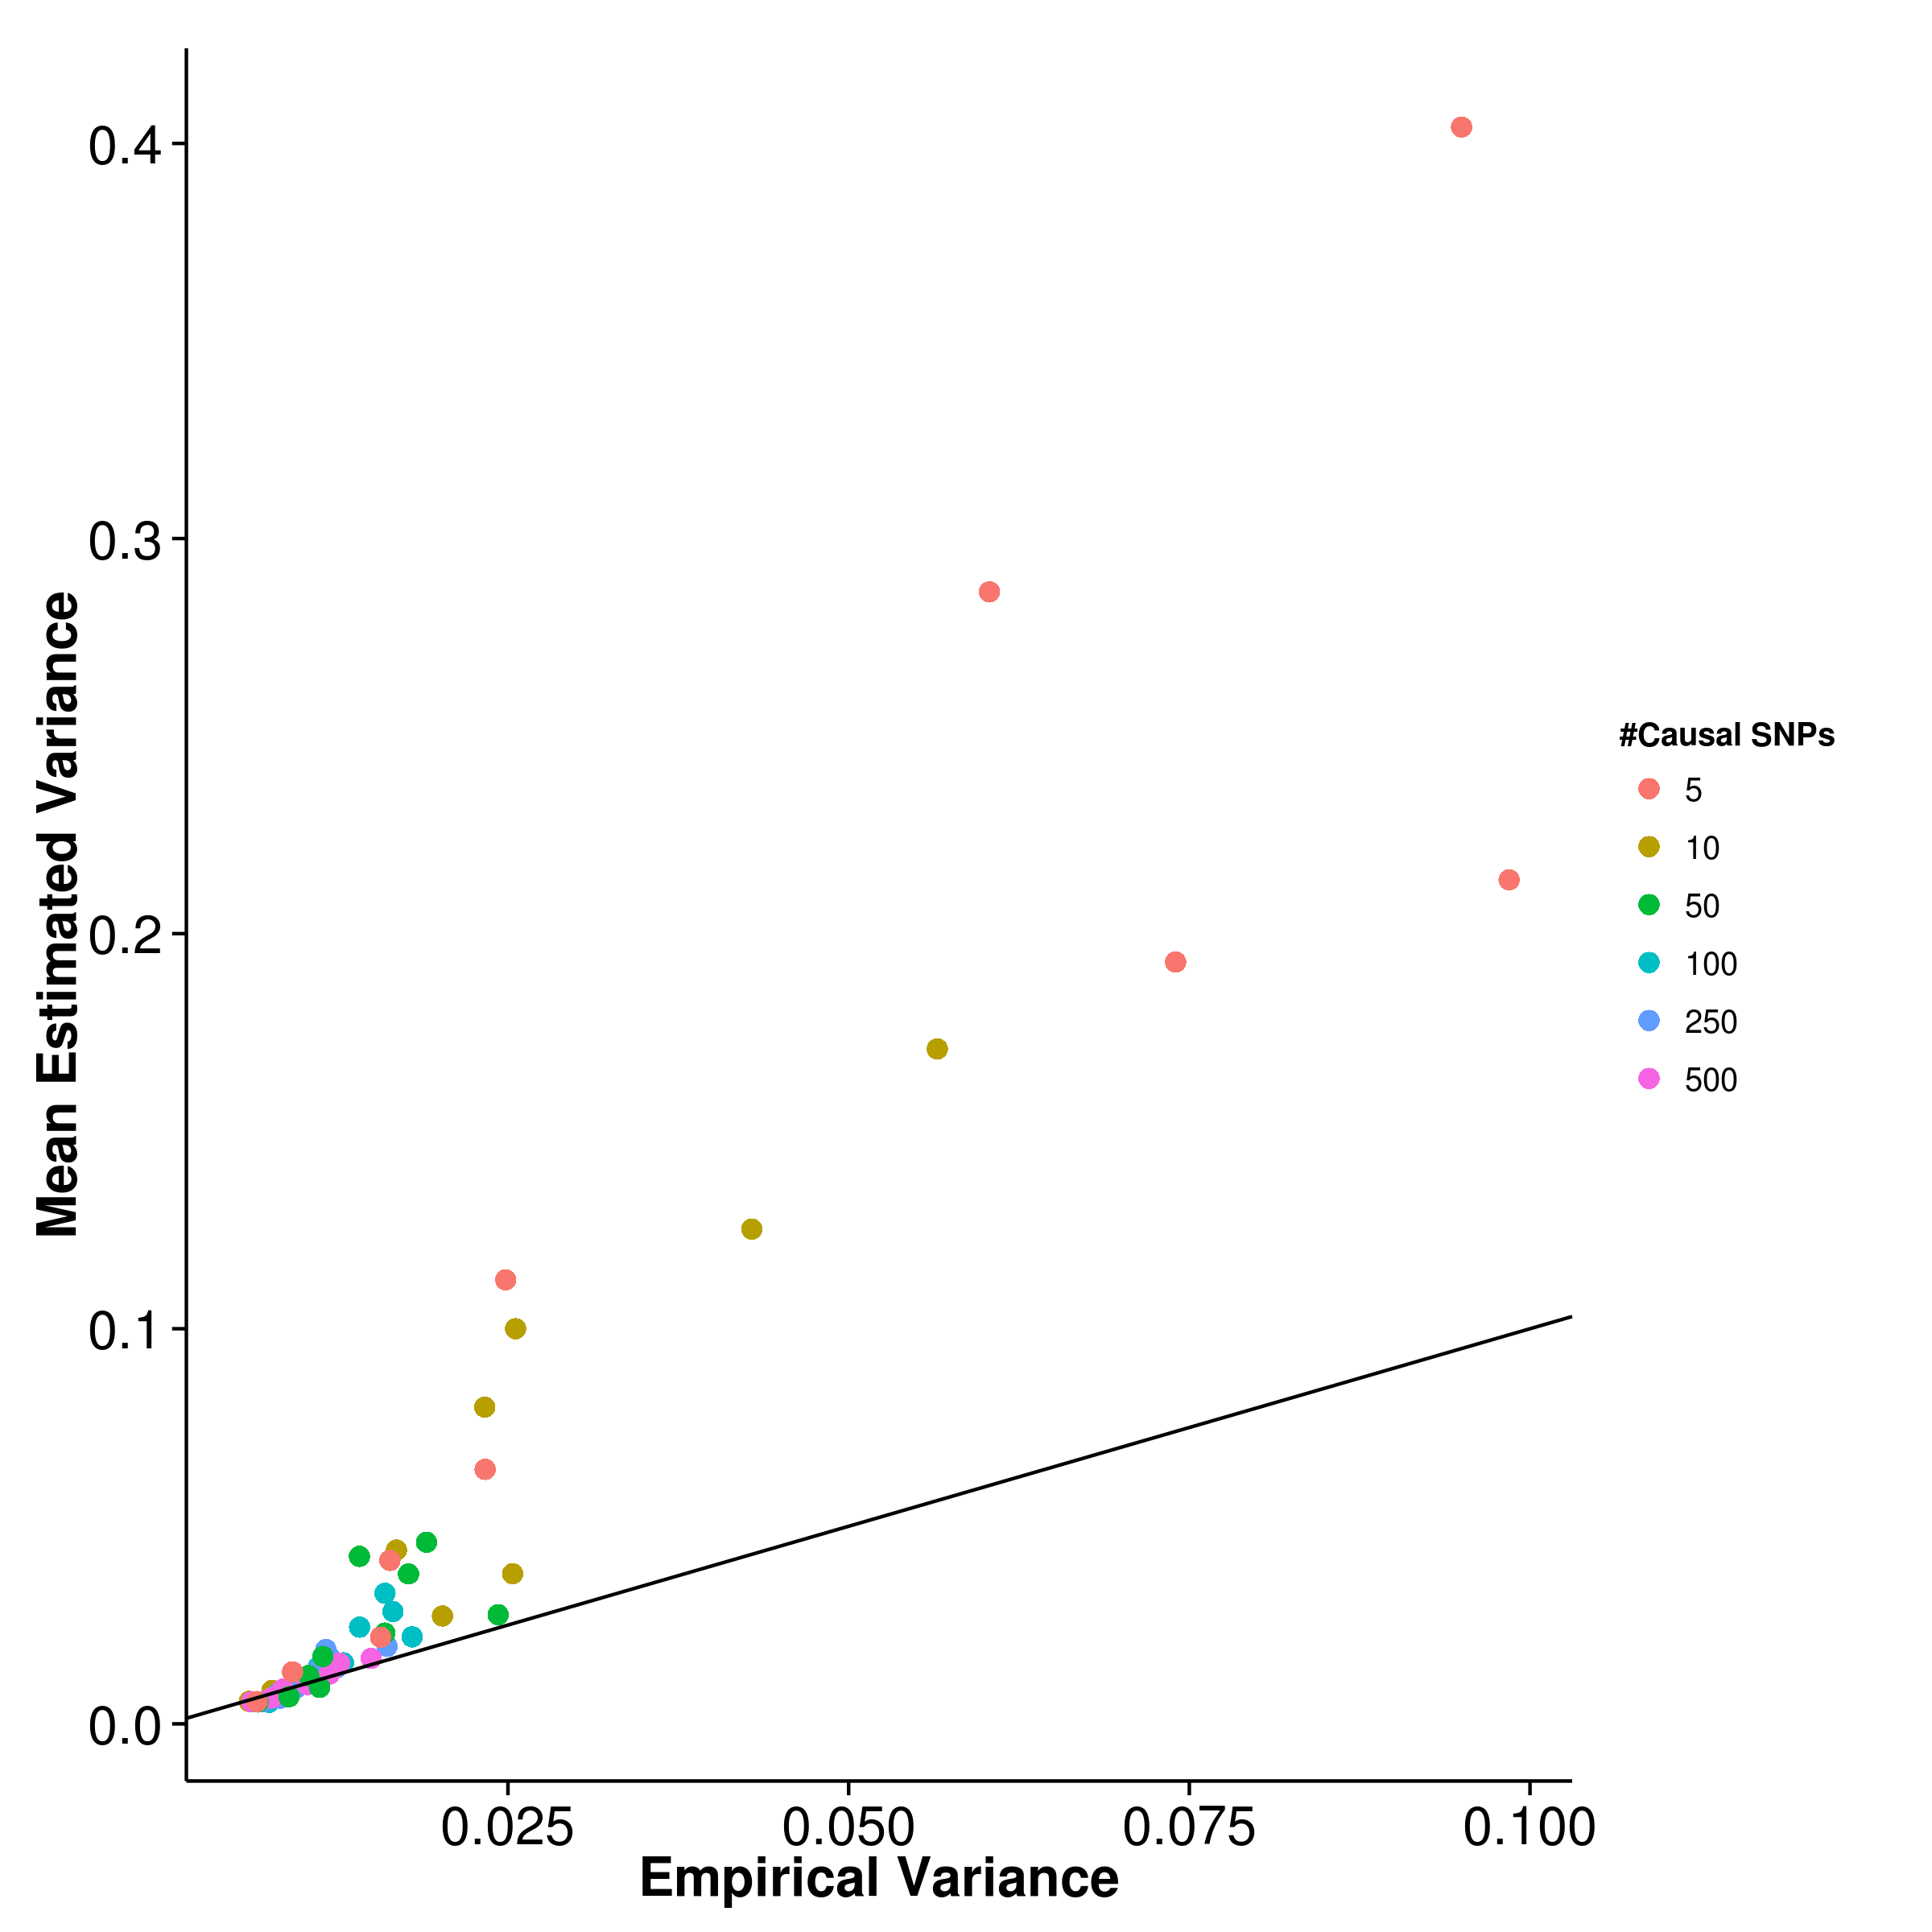
\includegraphics{figure/he_summary/random/ldsc_Qt_Random_sdCom.png}}
				\label{fig:ldscQtRandVarCom}
			}
			\subfloat[LDSC with intercept estimation]{
				
				\scalebox{.4}{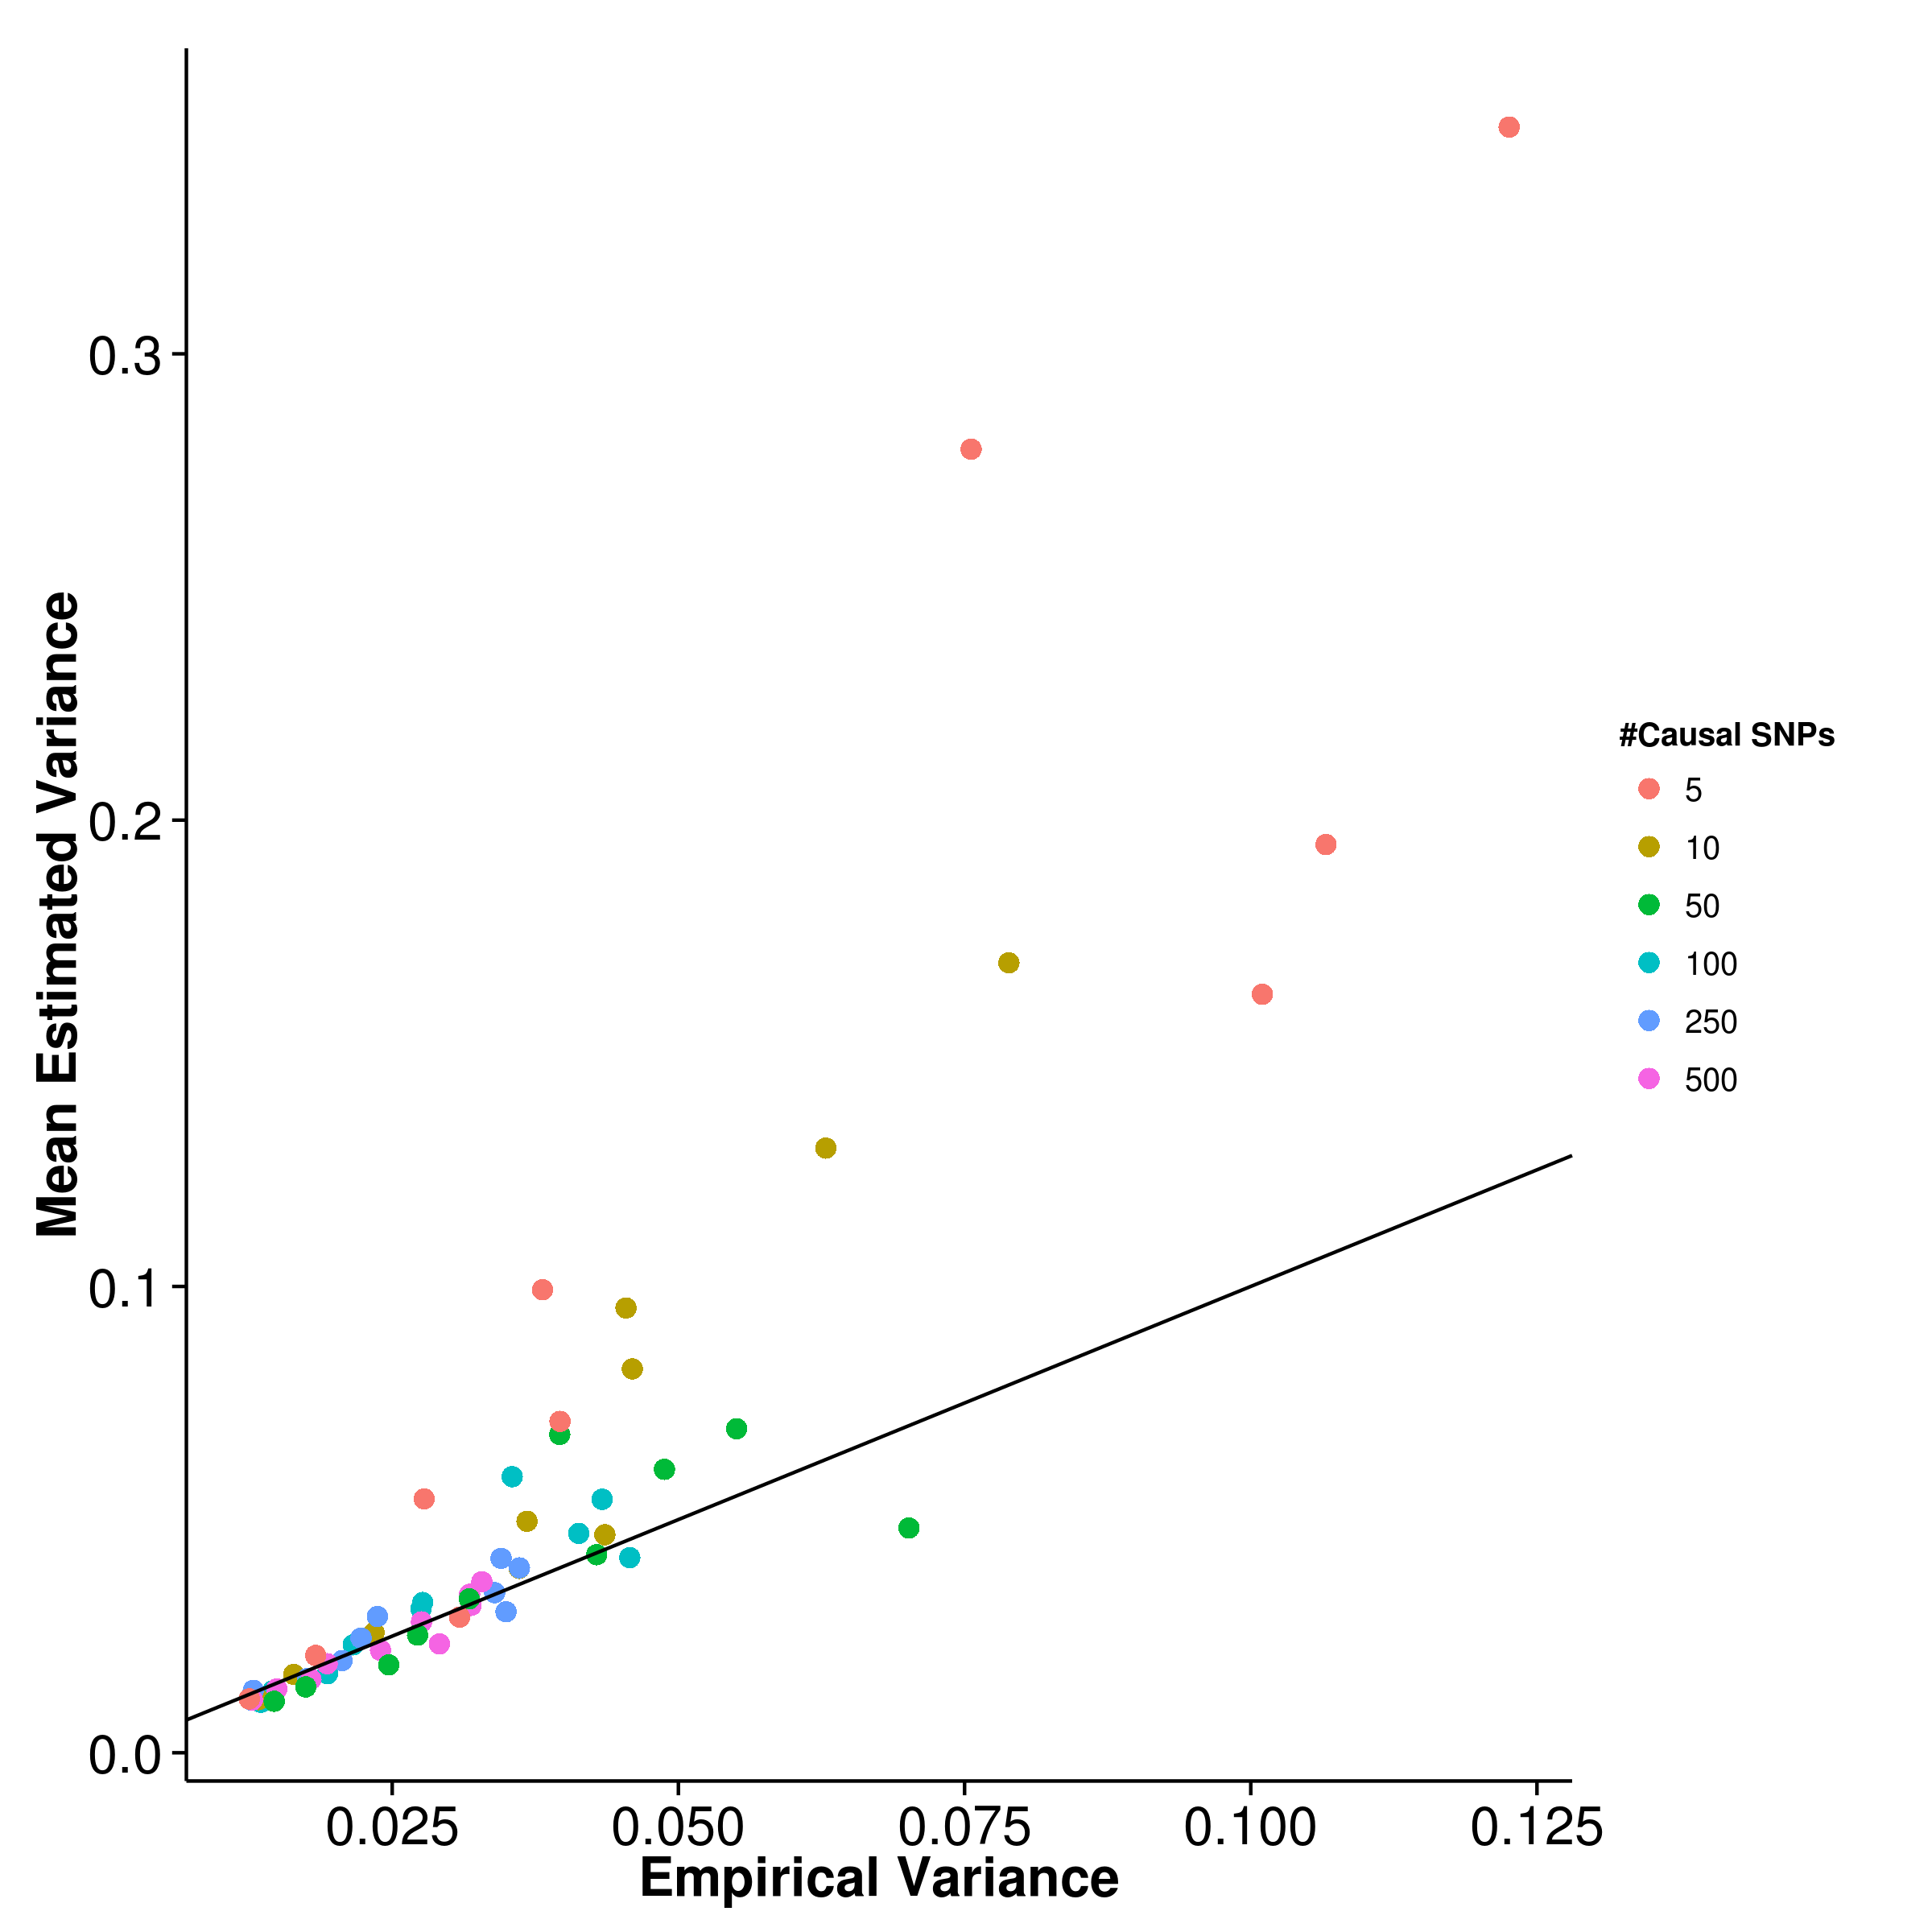
\includegraphics{figure/he_summary/random/ldscIn_Qt_Random_sdCom.png}}
				\label{fig:ldscInQtRandVarCom}
			}
			\caption[Quantitative Trait with Random Effect Size Simulation Result(Estimated Variance)]
			{Estimated variance of results from quantitative trait simulation with random effect size simulation when compared to the empirical variance.
			\gls{gcta} has the best estimate of its empirical variance whereas \gls{shrek} tends to under-estimate its empirical variance.
			On the other hand, \gls{ldsc} to over-estimate the variance especially when the number of causal \glspl{SNP} is small.
				} 
			\label{fig:QtRandVarCom}
		\end{figure}